Sau quá trình thực hiện luận văn, bằng cách sử dụng những công nghệ và kiến thức được đưa ra trong các phần trước, nhóm đã hoàn thành một Hệ thống quản lí vải nhuộm tương đối hoàn chỉnh.\par

Tài liệu về các API nhóm đã hiện thực và sử dụng trong hệ thống: \href{http://bit.ly/api-lvtn-202}{API Documentations [http://bit.ly/api-lvtn-202]}

Phần sau đây nhóm sẽ trình bày về giao diện ứng dụng mà nhóm hiện thực, cũng như hướng giải quyết các vấn đề gặp phải trong khi hiện thực. Và đây là địa chỉ dẫn đến trang web của nhóm: \href{https://fabric-management.herokuapp.com}{Quản lí vải nhuộm [https://fabric-management.herokuapp.com]}

%%%%%%%%%%%%%%%%%%%%%%%%
\textbf{Trang đăng nhập}

Sau khi được Quản lí cung cấp tài khoản, nhân viên có thể đăng nhập vào hệ thống ở trang Đăng nhập [Hình \ref{result_dang_nhap}]. Sau khi đăng nhập thành công, tài khoản này sẽ được server cung cấp một token để thực hiện các yêu cầu API xuyên suốt trong quá trình xử dụng ứng dụng. Token sẽ hết hạn nếu như sau 30 phút không có bất cứ yêu cầu nào lên server, khi này người dùng cần đăng nhập lại để tiếp tục sử dụng.\par
Token được lưu trữ ở Local Storage, việc lưu trữ nằm nhằm mục đích khi người dùng tải lại trang, tất cả state của hệ thống sẽ bị xóa, khi này sẽ lấy token đã lưu để lấy lại thông tin mà không yêu cầu người dùng phải đăng nhập lại.
\begin{figure}[H]
    \begin{center}
        \frame{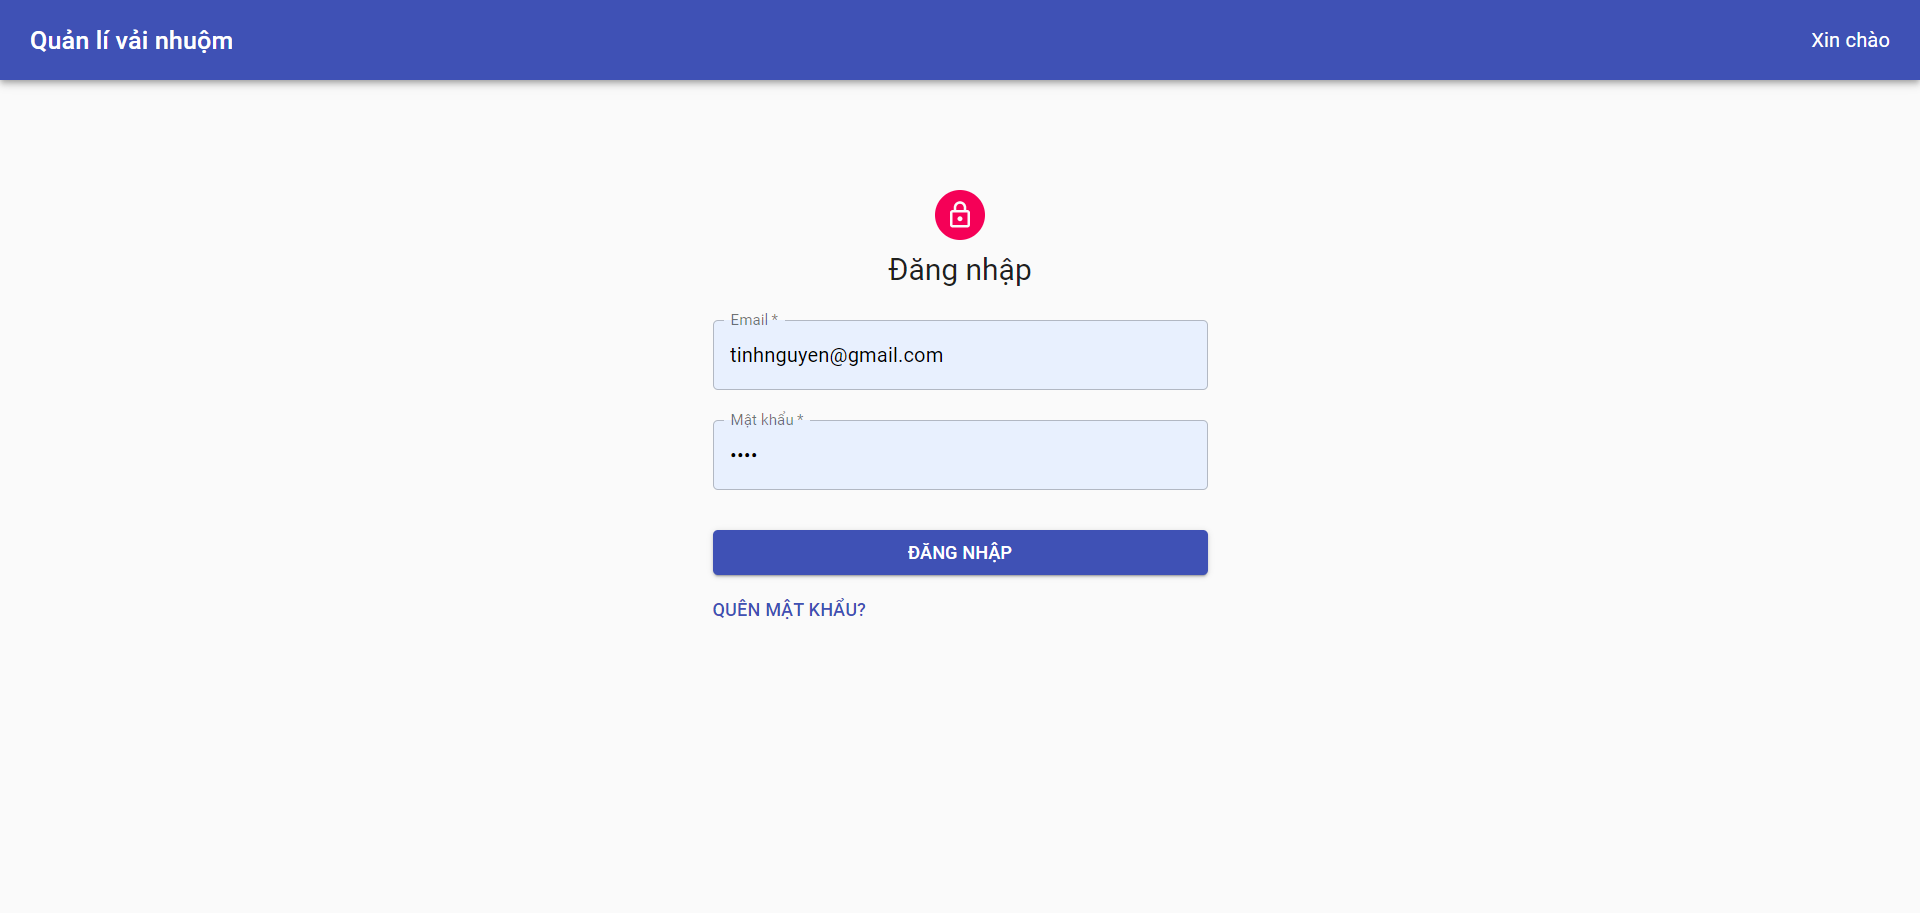
\includegraphics[width=14cm]{Image/result/dang_nhap.png}}
        \caption{Giao diện trang đăng nhập}
        \label{result_dang_nhap}
    \end{center}
\end{figure}

%%%%%%%%%%%%%%%%%%%%%%%%
\textbf{Khôi phục mật khẩu}

Người dùng quên mật khẩu, có thể yêu cầu cập nhật mật khẩu mới bằng cách nhấn vào dòng chứ "Quên mật khẩu" phía dưới nút Đăng nhập, khi này sẽ được chuyển sang trang Nhập Email. [Hình \ref{result_quen_mat_khau_email}]\par
Khi người dùng nhập xong và nhấn nút Gửi, một email sẽ được gửi đi, trong email sẽ có một đường dẫn để dẫn đến trang cập nhật mật khẩu mới [Hình \ref{result_quen_mat_khau_email_receive}]. Trong đường dẫn này, nhóm có chèn một token vào, token này dùng để định dạng người dùng nào đang yêu cầu, và sẽ được gửi lên server cùng với mật khẩu mới. Token có thời hạn là 5 phút, sau khi hết hạn, nếu người dùng truy cập vào đường dẫn này thì sẽ được chuyển sang trang Đăng nhập, lúc này cần phải thực hiện lại yêu cầu cập nhật mật khẩu.\par
Cuối cùng, người dùng nhập mật khẩu mới của mình vào để cập nhật. [Hình \ref{result_quen_mat_khau_new_password}]

\begin{figure}[H]
    \begin{center}
        \frame{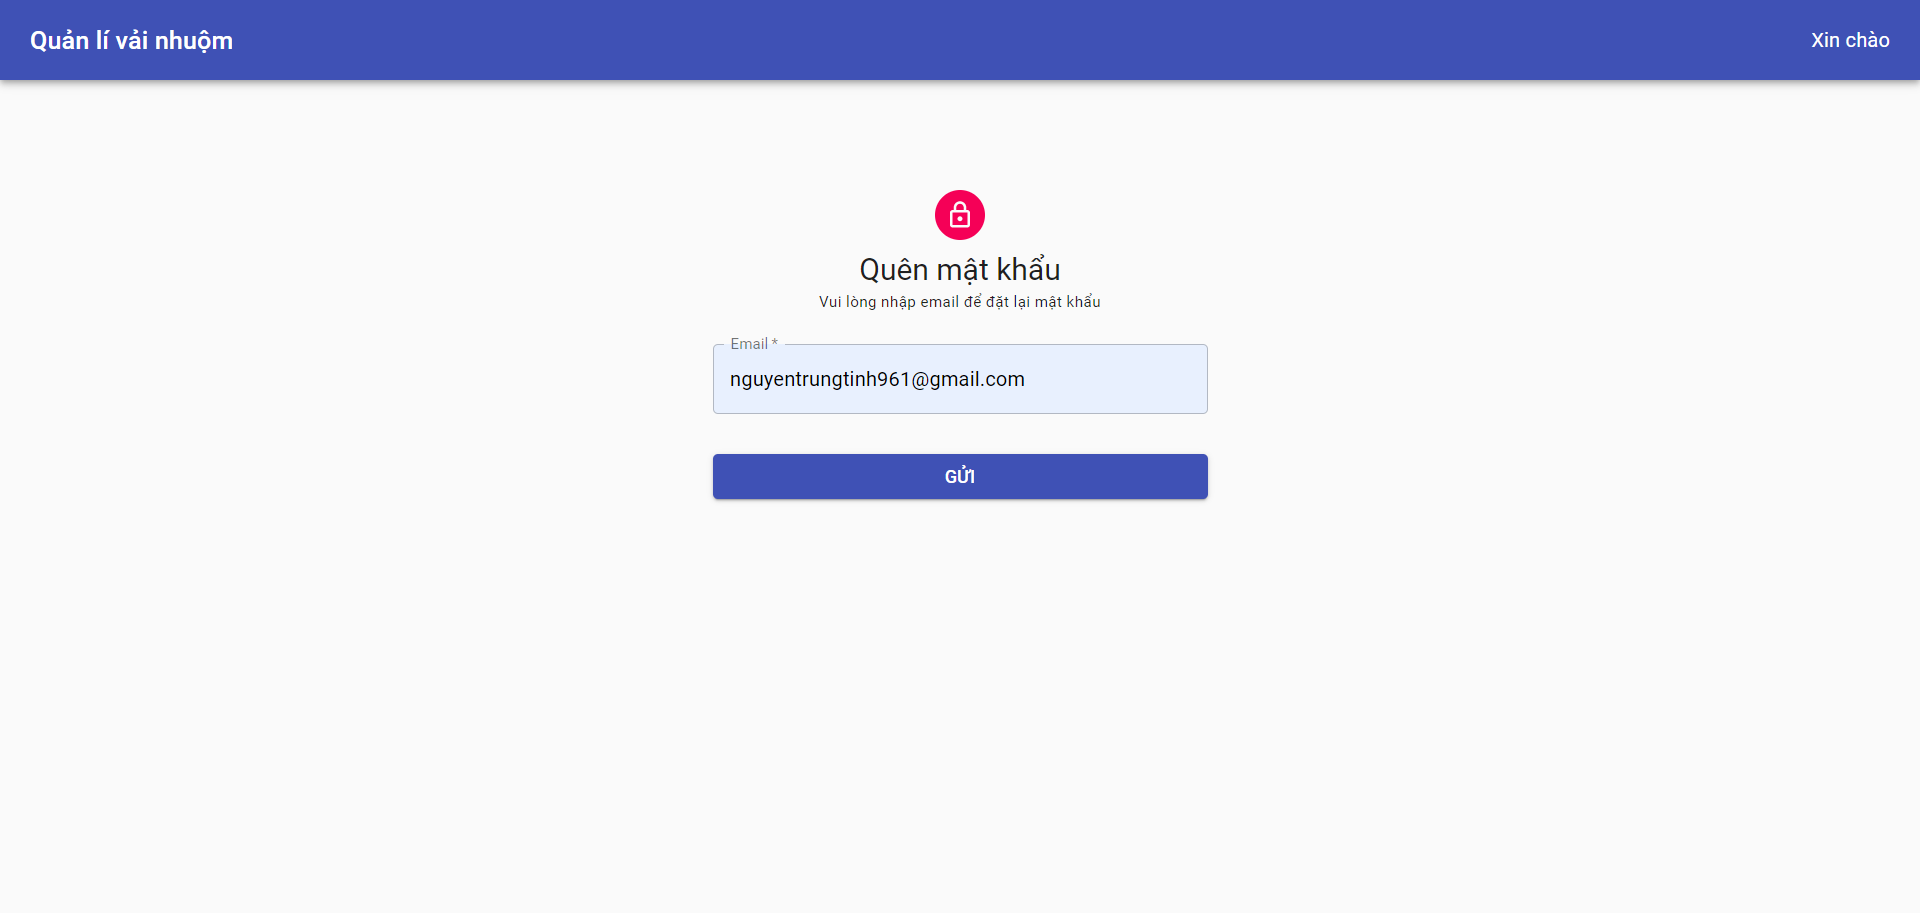
\includegraphics[width=14cm]{Image/result/quen_mat_khau_email.png}}
        \caption{Giao diện trang Quên mật khẩu}
        \label{result_quen_mat_khau_email}
    \end{center}
\end{figure}

\begin{figure}[H]
    \begin{center}
        \frame{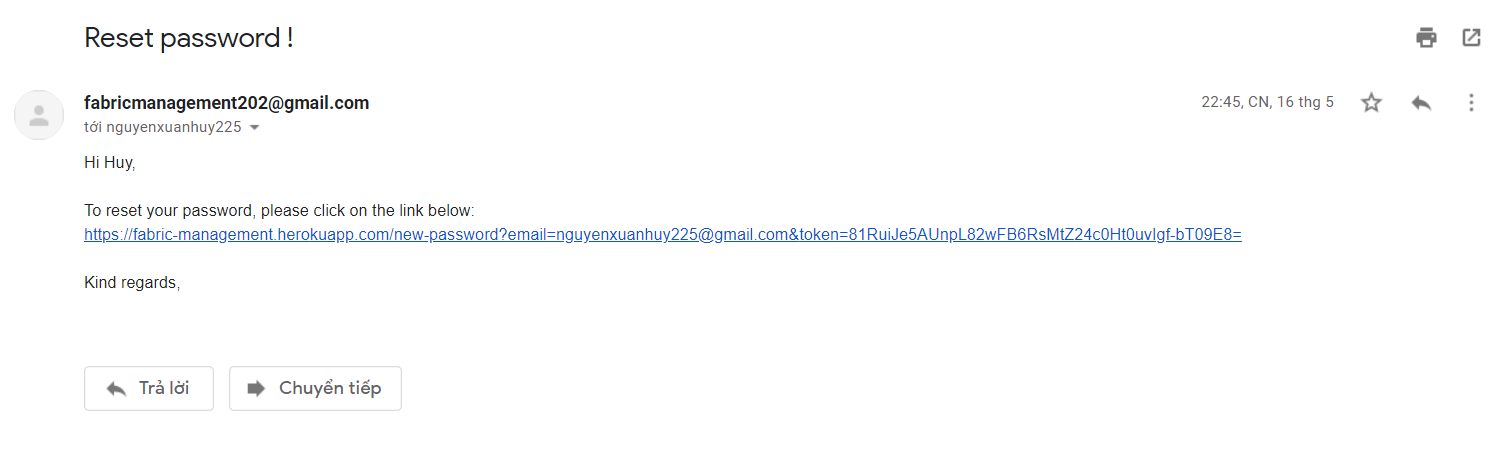
\includegraphics[width=14cm]{Image/result/quen_mat_khau_gmail.png}}
        \caption{Email người dùng nhận được}
        \label{result_quen_mat_khau_email_receive}
    \end{center}
\end{figure}

\begin{figure}[H]
    \begin{center}
        \frame{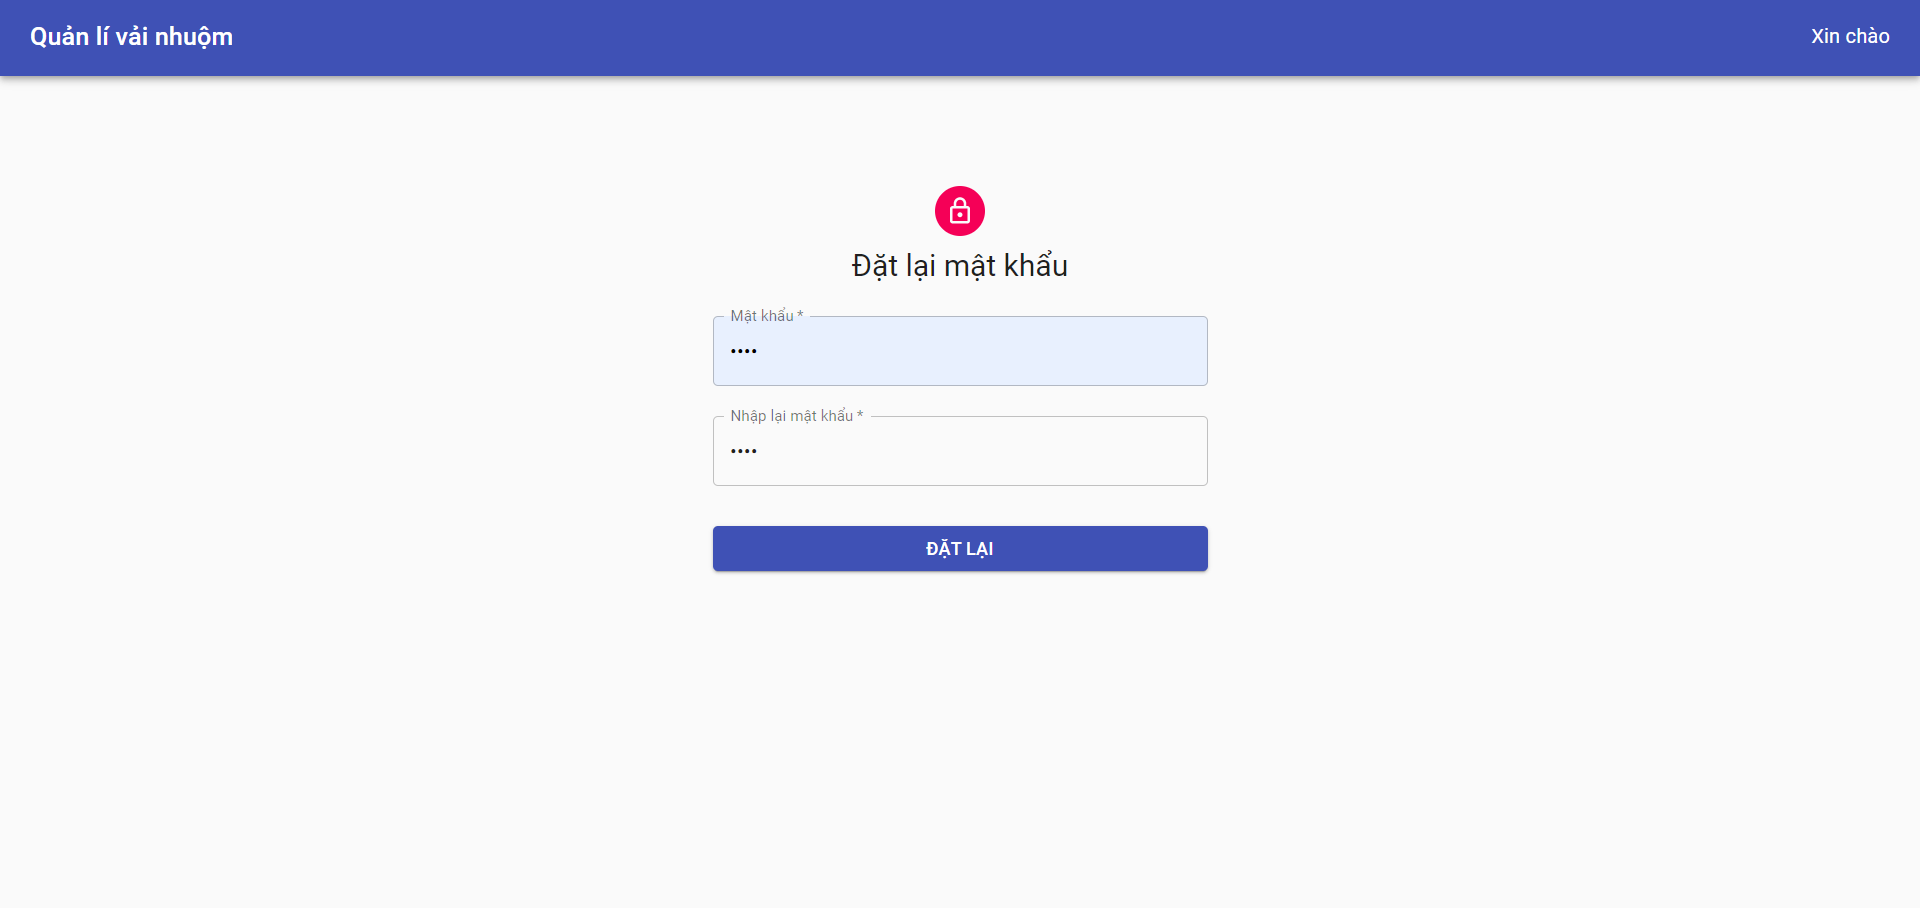
\includegraphics[width=14cm]{Image/result/quen_mat_khau_new_password}}
        \caption{Giao diện trang Nhập mật khẩu mới}
        \label{result_quen_mat_khau_new_password}
    \end{center}
\end{figure}


%%%%%%%%%%%%%%%%%%%%%%%%
\textbf{Dashboard}

Trang này tổng hợp một số thông tin thống kê gần đây của hệ thống và hiển thị dưới dạng biểu đồ và các bảng biểu. [Hình \ref{result_dashboard}] \par

Với biểu đồ \textbf{Thống kê sản lượng trong năm}, ta có thể thấy được sản lượng vải mà các xưởng đã nhuộm được trong năm vừa qua. Từ đó có thể đánh giá được tháng nào, quý nào mà xưởng nhuộm làm việc không hiệu quả. \par

Với biểu đồ \textbf{Thống kê vải thành phẩm}, ta sẽ có được các nhìn trực quan số lượng vải thành phẩm được nhuộm trong một khoảng thời gian, được so sánh theo xưởng và theo loại vải. \par

Với ba thống kê còn lại là \textbf{Thanh toán gần đây, Phiếu nhập gần đây, Phiếu xuất gần đây} liệt kê ra thông tin các hoạt động gần đây của doanh nghiệp. \par

\begin{figure}[H]
    \begin{center}
        \frame{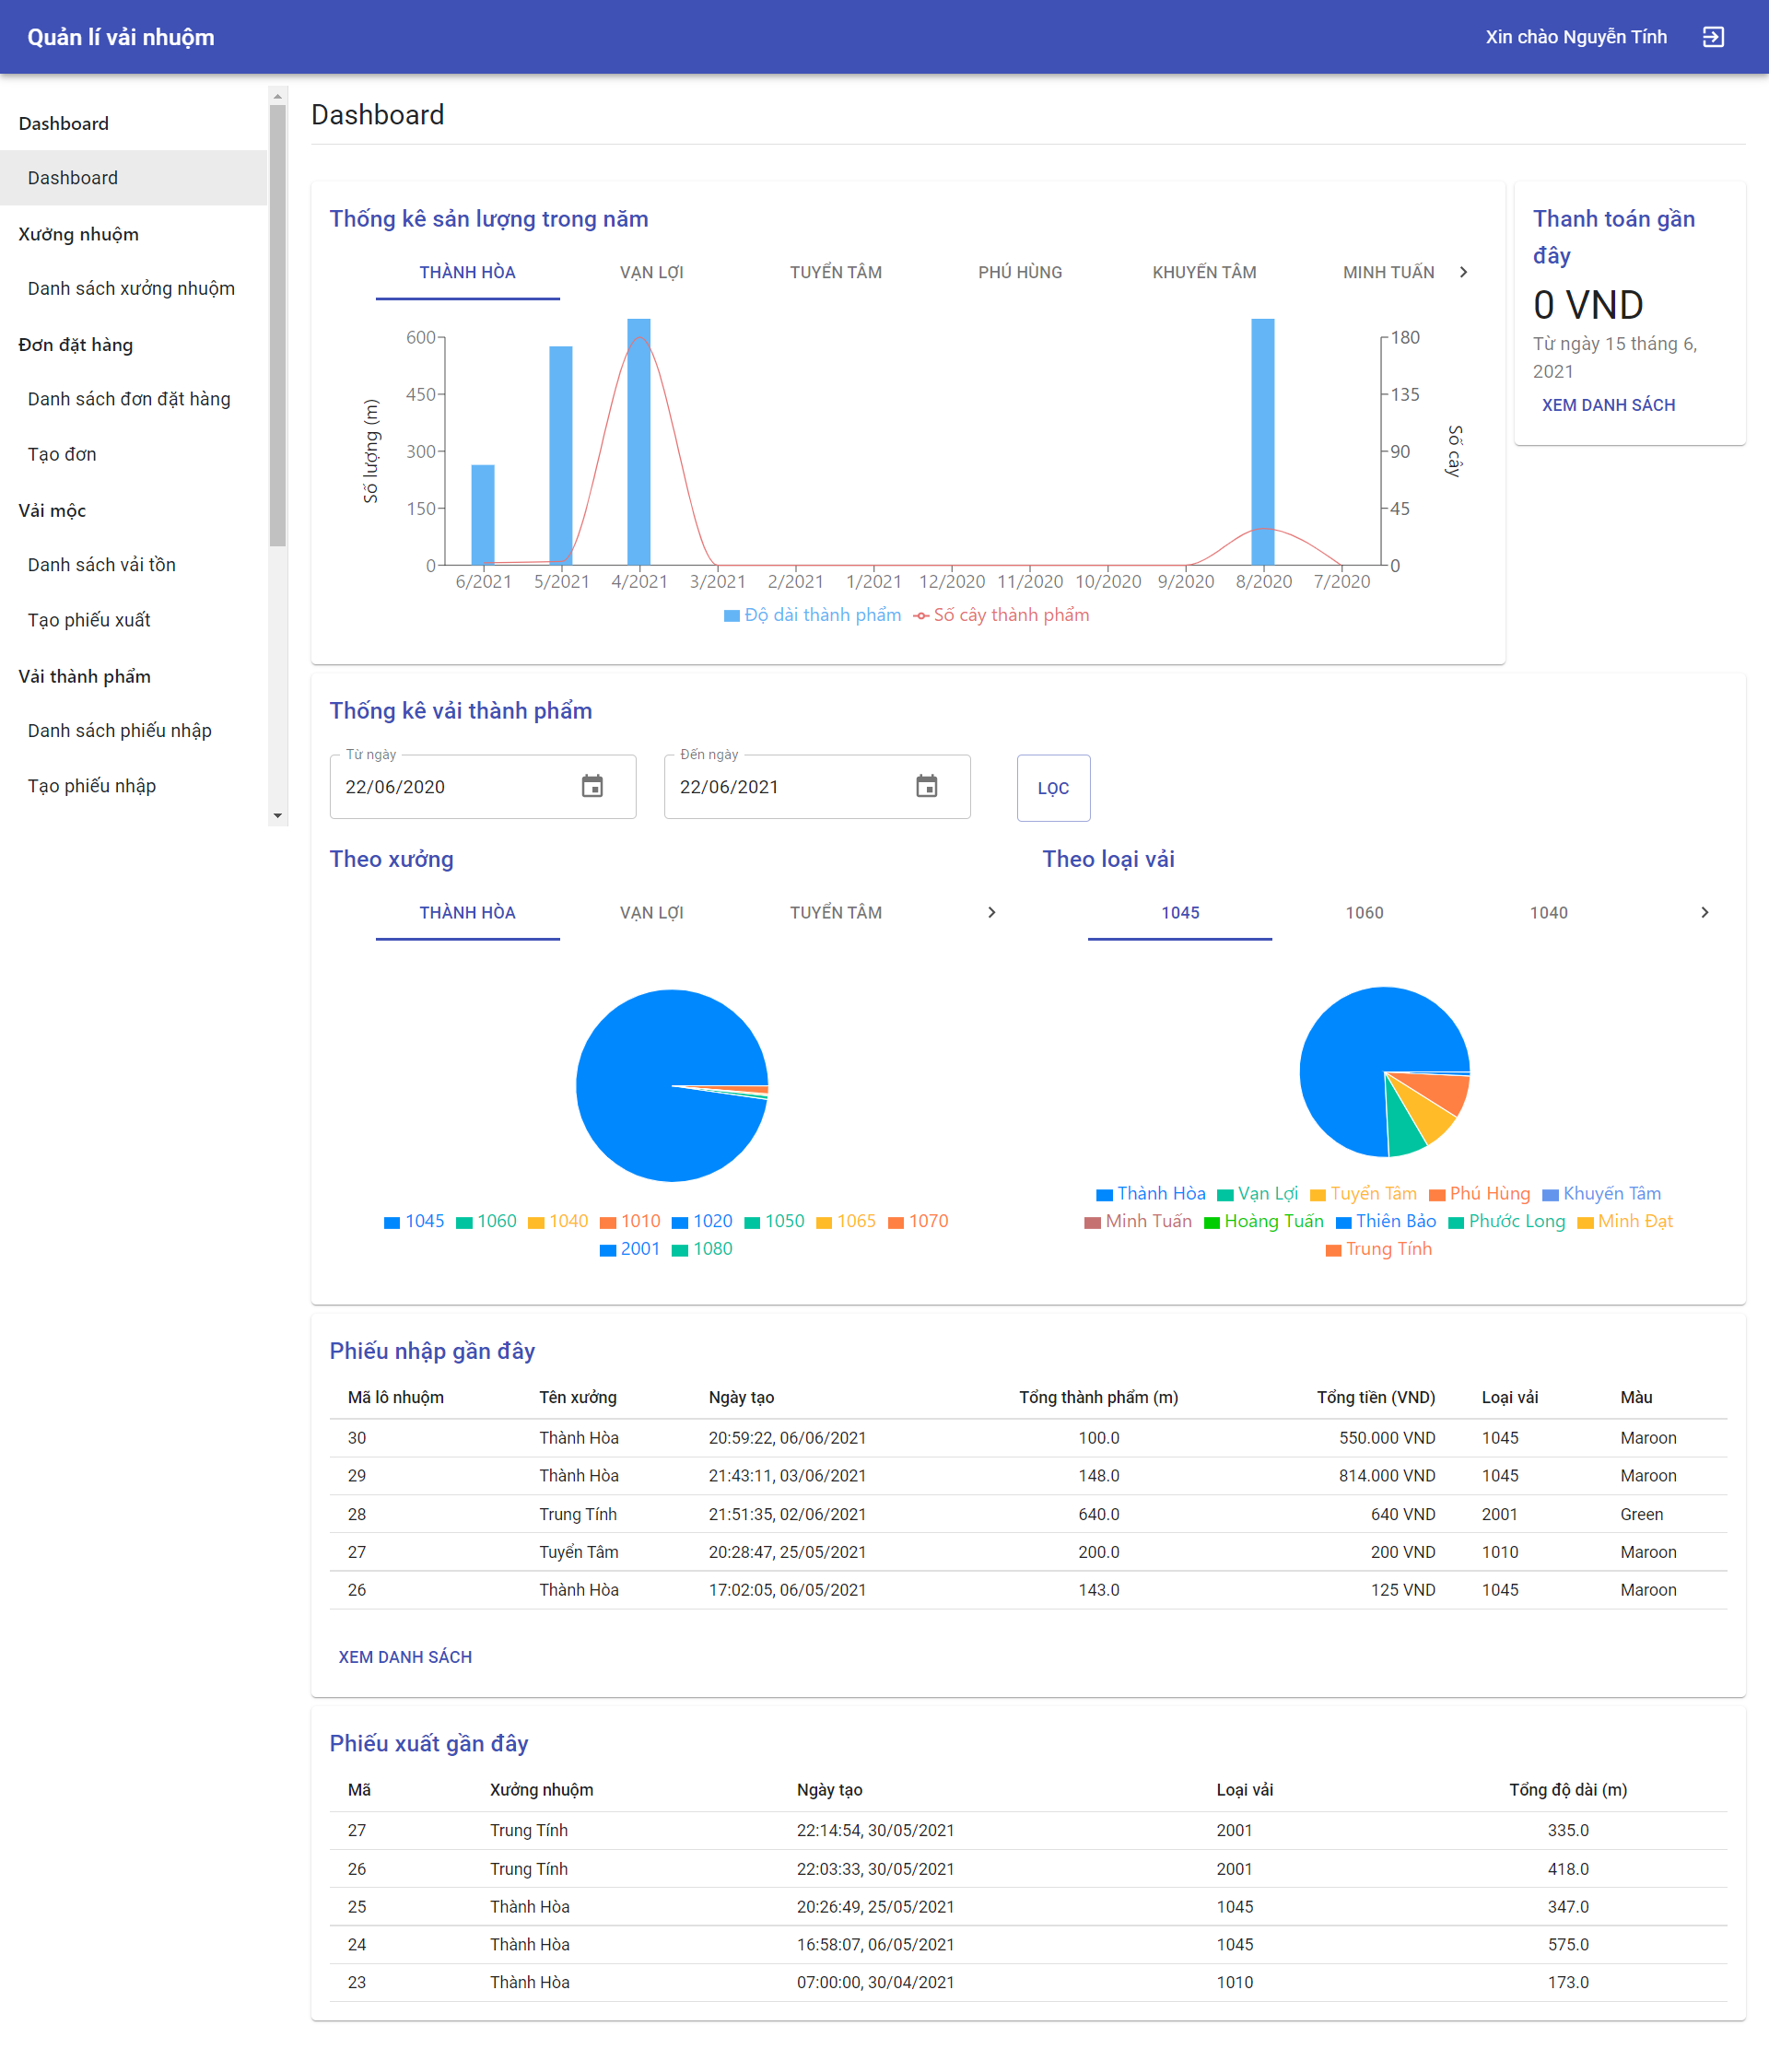
\includegraphics[width=14cm]{Image/result/dashboard.png}}
        \caption{Giao diện trang Dashboard}
        \label{result_dashboard}
    \end{center}
\end{figure}

%%%%%%%%%%%%%%%%%%%%%%%%
\textbf{Quản lí xưởng nhuộm}

Ở nhóm chức năng này, người dùng có thể xem danh sách các xưởng nhuộm [Hình \ref{result_danh_sach_xuong}], xem thông tin chi tiết của xưởng nhuộm bao gồm các đơn đặt hàng của xưởng nhuộm đó [Hình \ref{result_chi_tiet_xuong}], chỉnh sửa các thông tin của xưởng [Hình \ref{result_sua_thong_tin_xuong}], và xem thống kê danh sách vải mộc tồn kho và vải thành phẩm xưởng đã nhuộm. [Hình \ref{result_ton_kho_xuong}]\par

Trong trang Chi tiết xưởng nhuộm, có bốn nút tương ứng với các hành động sau: 
\begin{itemize}
    \item Chỉnh sửa thông tin: mở pop-up chỉnh sửa thông tin xưởng.
    \item Tạo đơn đặt hàng: chuyển sang trang Tạo đơn đặt hàng mới của xưởng này.
    \item Tạo thanh toán: tạo hóa đơn thanh toán công nợ của xưởng.
    \item Danh sách hàng tồn: xem danh sách vải mộc tồn kho ở xưởng.
\end{itemize}

Ngoài ra, khi nhấn vào các đơn đặt hàng trong Danh sách đơn đặt hàng sẽ chuyển sang trang Chi tiết đơn đặt hàng đó.

\begin{figure}[H]
    \begin{center}
        \frame{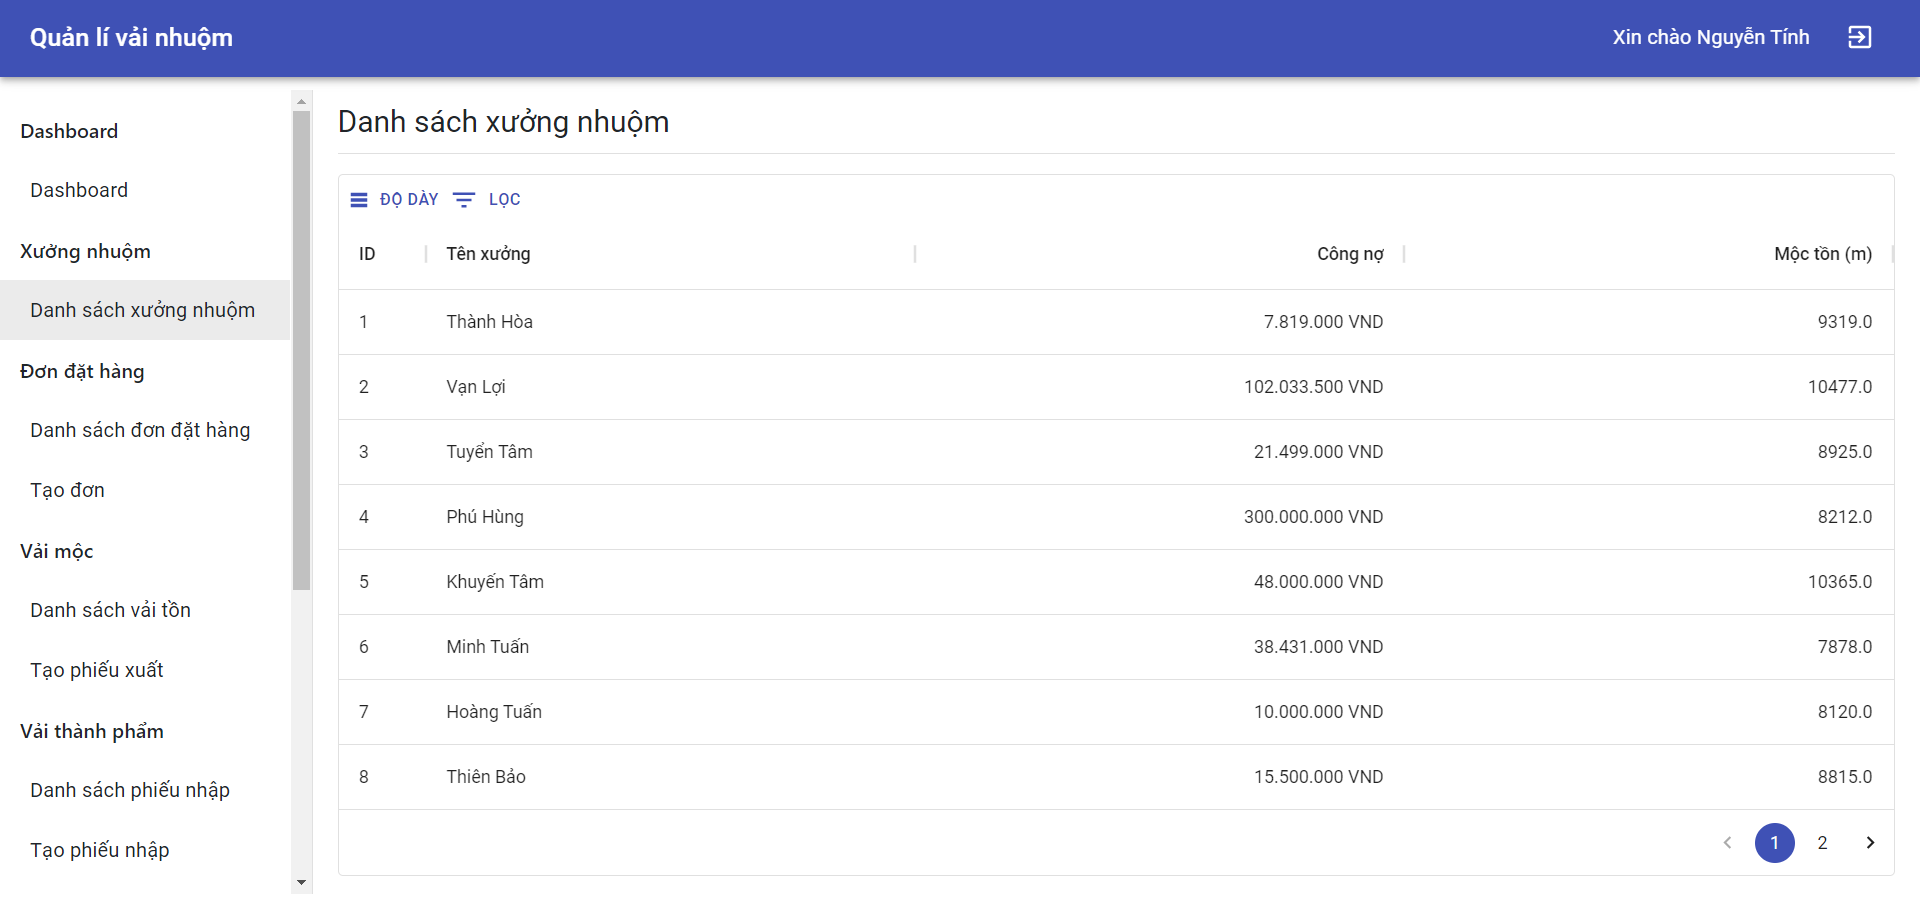
\includegraphics[width=14cm]{Image/result/danh_sach_xuong.png}}
        \caption{Giao diện trang Danh sách xưởng nhuộm}
        \label{result_danh_sach_xuong}
    \end{center}
\end{figure}

\begin{figure}[H]
    \begin{center}
        \frame{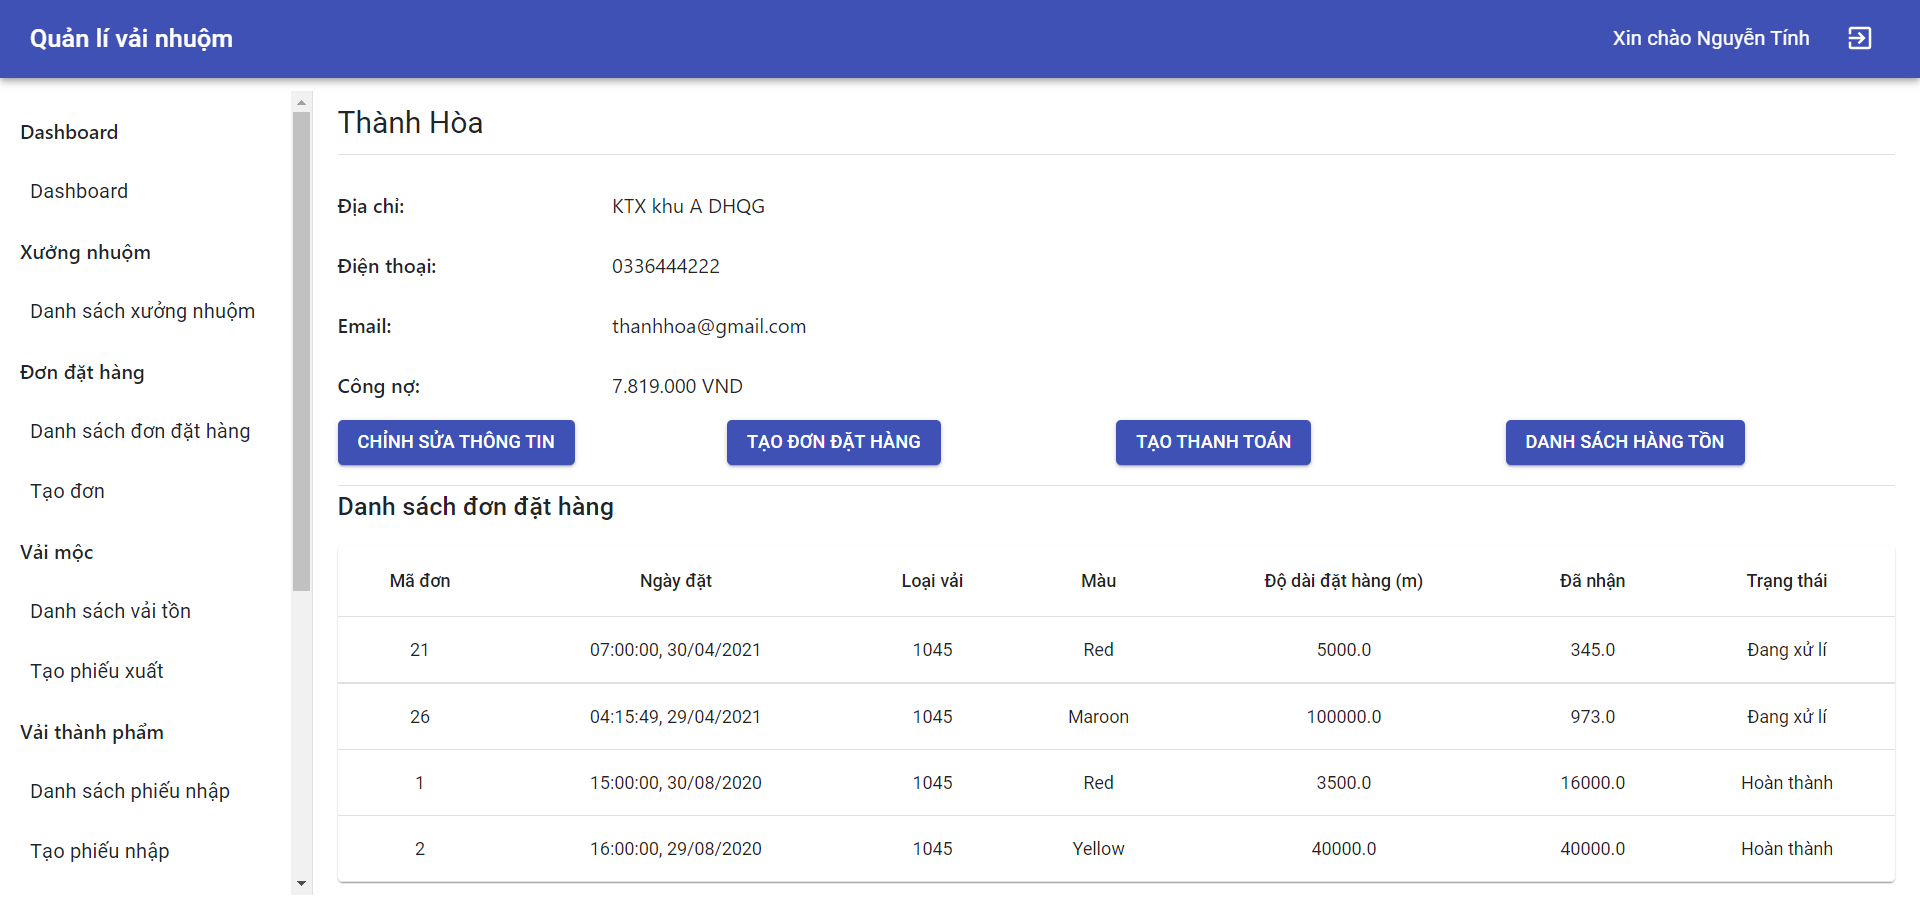
\includegraphics[width=14cm]{Image/result/chi_tiet_xuong.png}}
        \caption{Giao diện trang Chi tiết xưởng nhuộm}
        \label{result_chi_tiet_xuong}
    \end{center}
\end{figure}

\begin{figure}[H]
    \begin{center}
        \frame{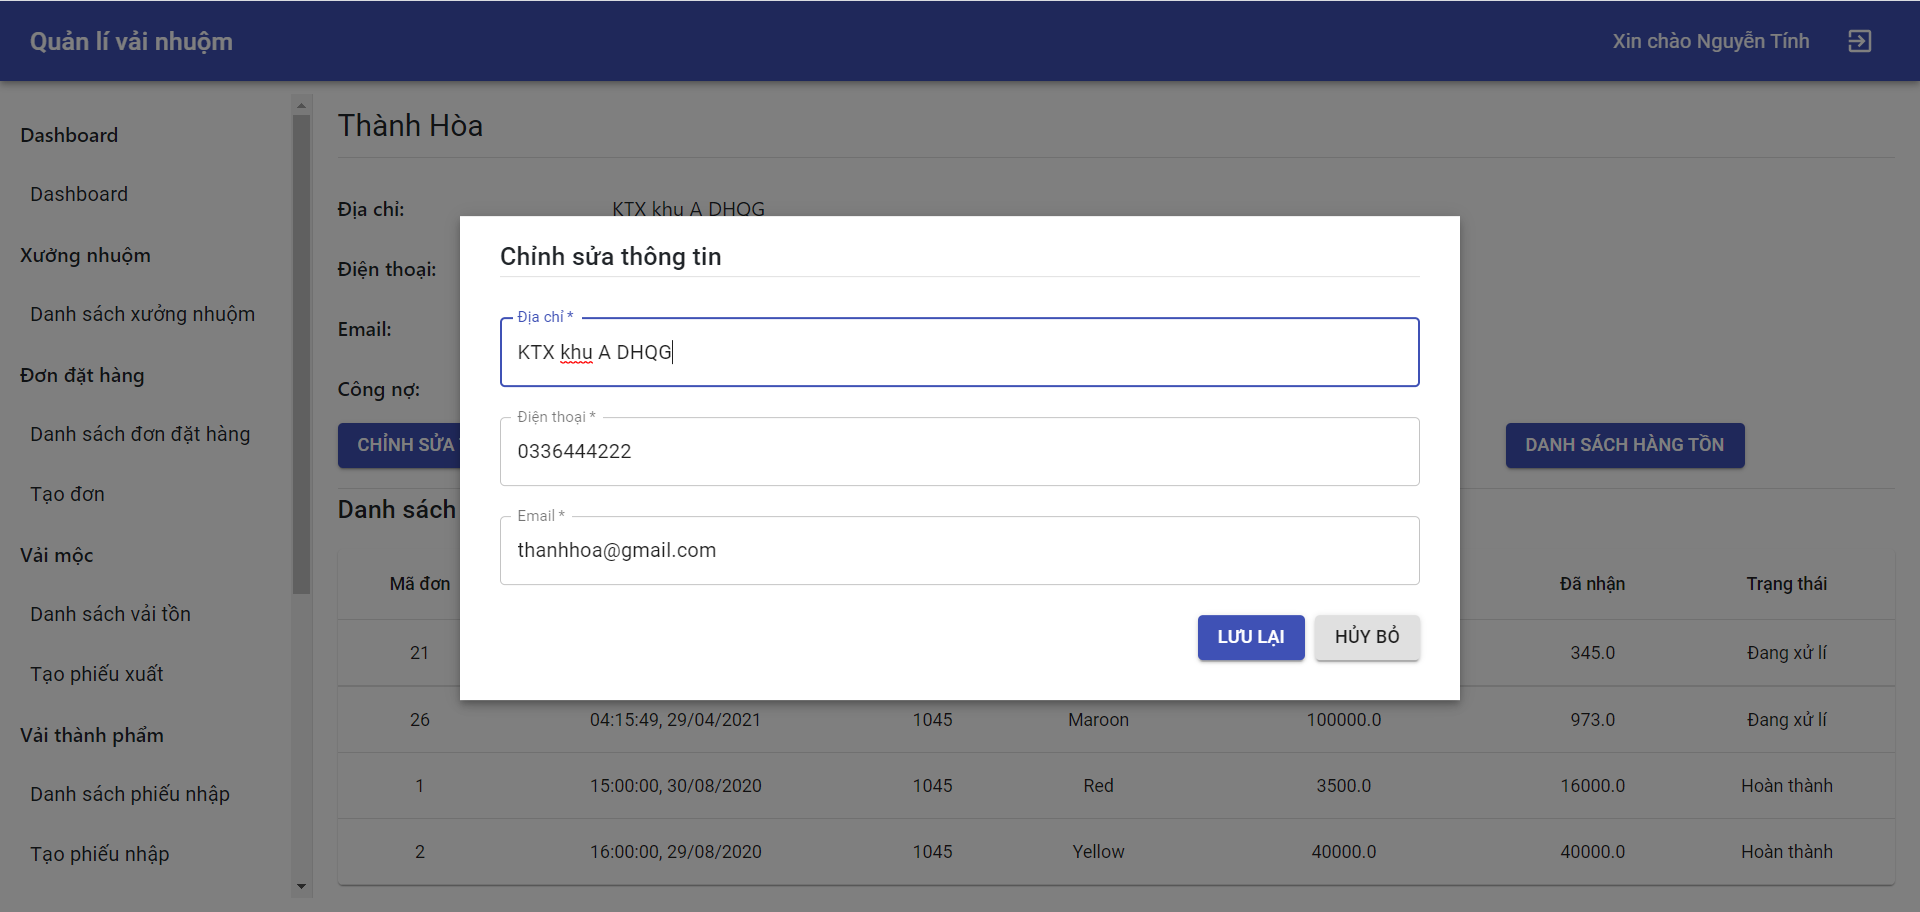
\includegraphics[width=14cm]{Image/result/sua_thong_tin_xuong.png}}
        \caption{Giao diện trang Chỉnh sửa thông tin xưởng}
        \label{result_sua_thong_tin_xuong}
    \end{center}
\end{figure}

\begin{figure}[H]
    \begin{center}
        \frame{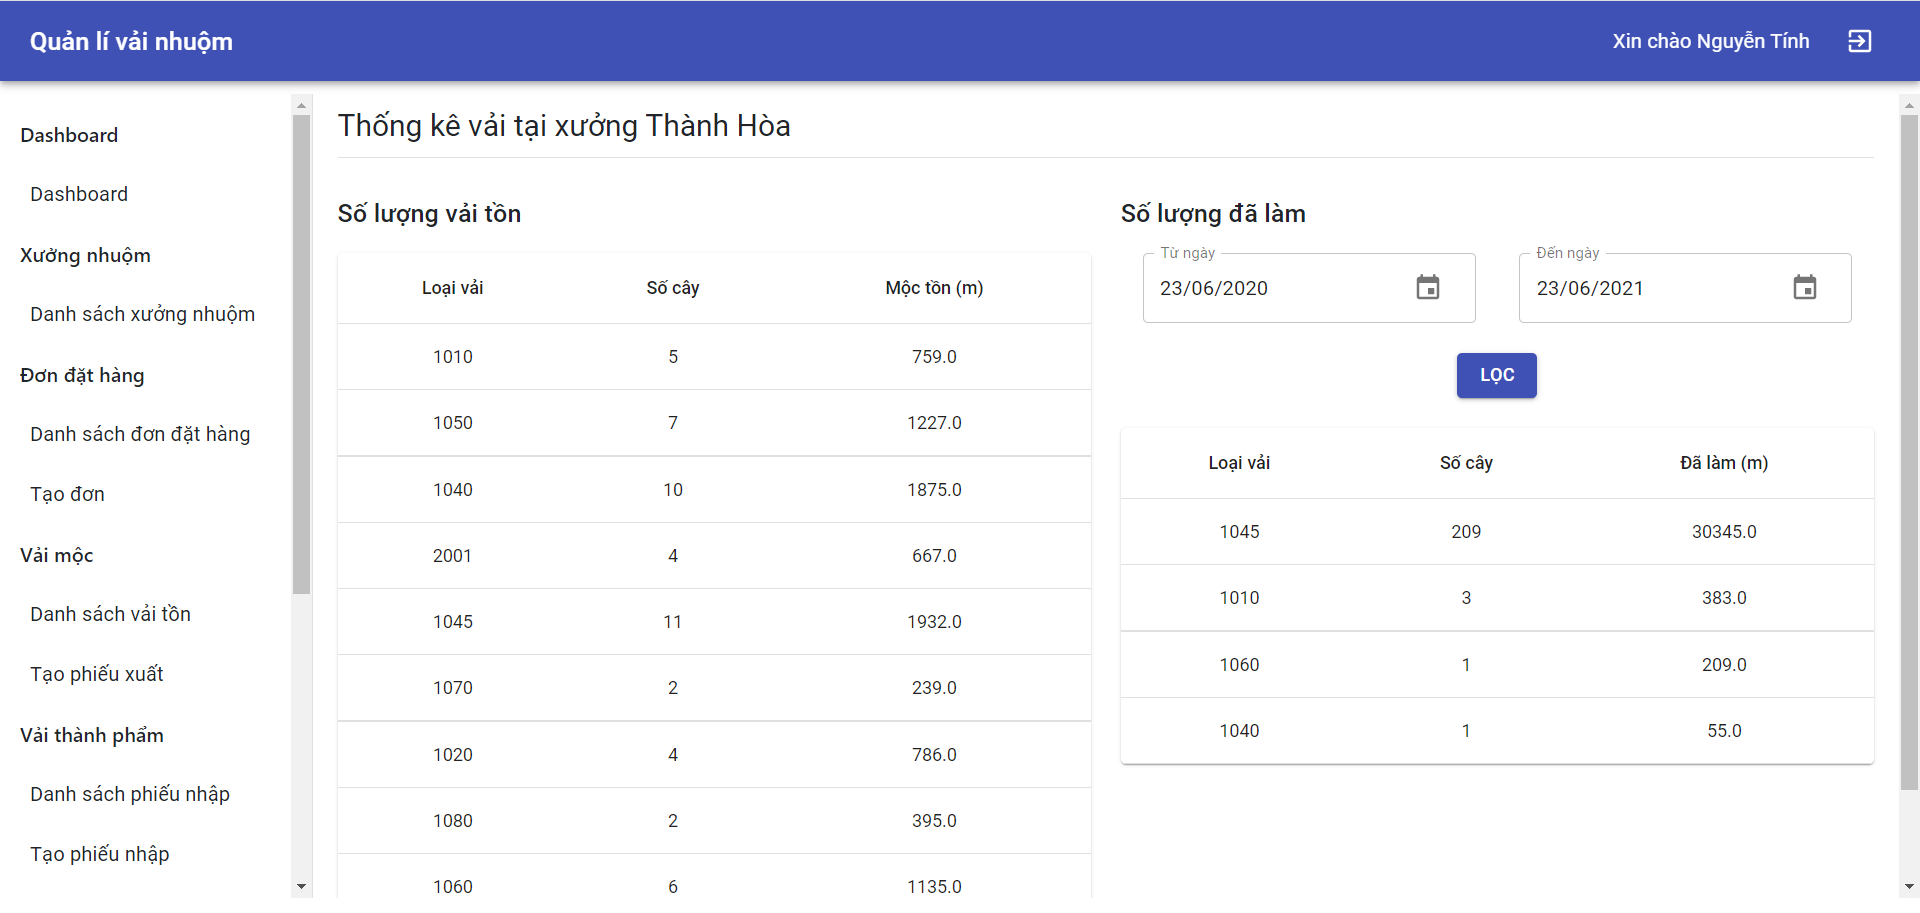
\includegraphics[width=14cm]{Image/result/ton_kho_xuong.png}}
        \caption{Giao diện trang Thống kê vải tại xưởng}
        \label{result_ton_kho_xuong}
    \end{center}
\end{figure}

%%%%%%%%%%%%%%%%%%%%%%%%
\textbf{Quản lí đơn đặt hàng}

Ở nhóm chức năng này, người dùng có thể xem danh sách các đơn đặt hàng [Hình \ref{result_danh_sach_don_hang}], thông tin chi tiết của đơn đặt hàng [Hình \ref{result_chi_tiet_don_hang}], và tạo một đơn đặt hàng mới [Hình \ref{result_tao_don_hang}]. \par

\begin{figure}[H]
    \begin{center}
        \frame{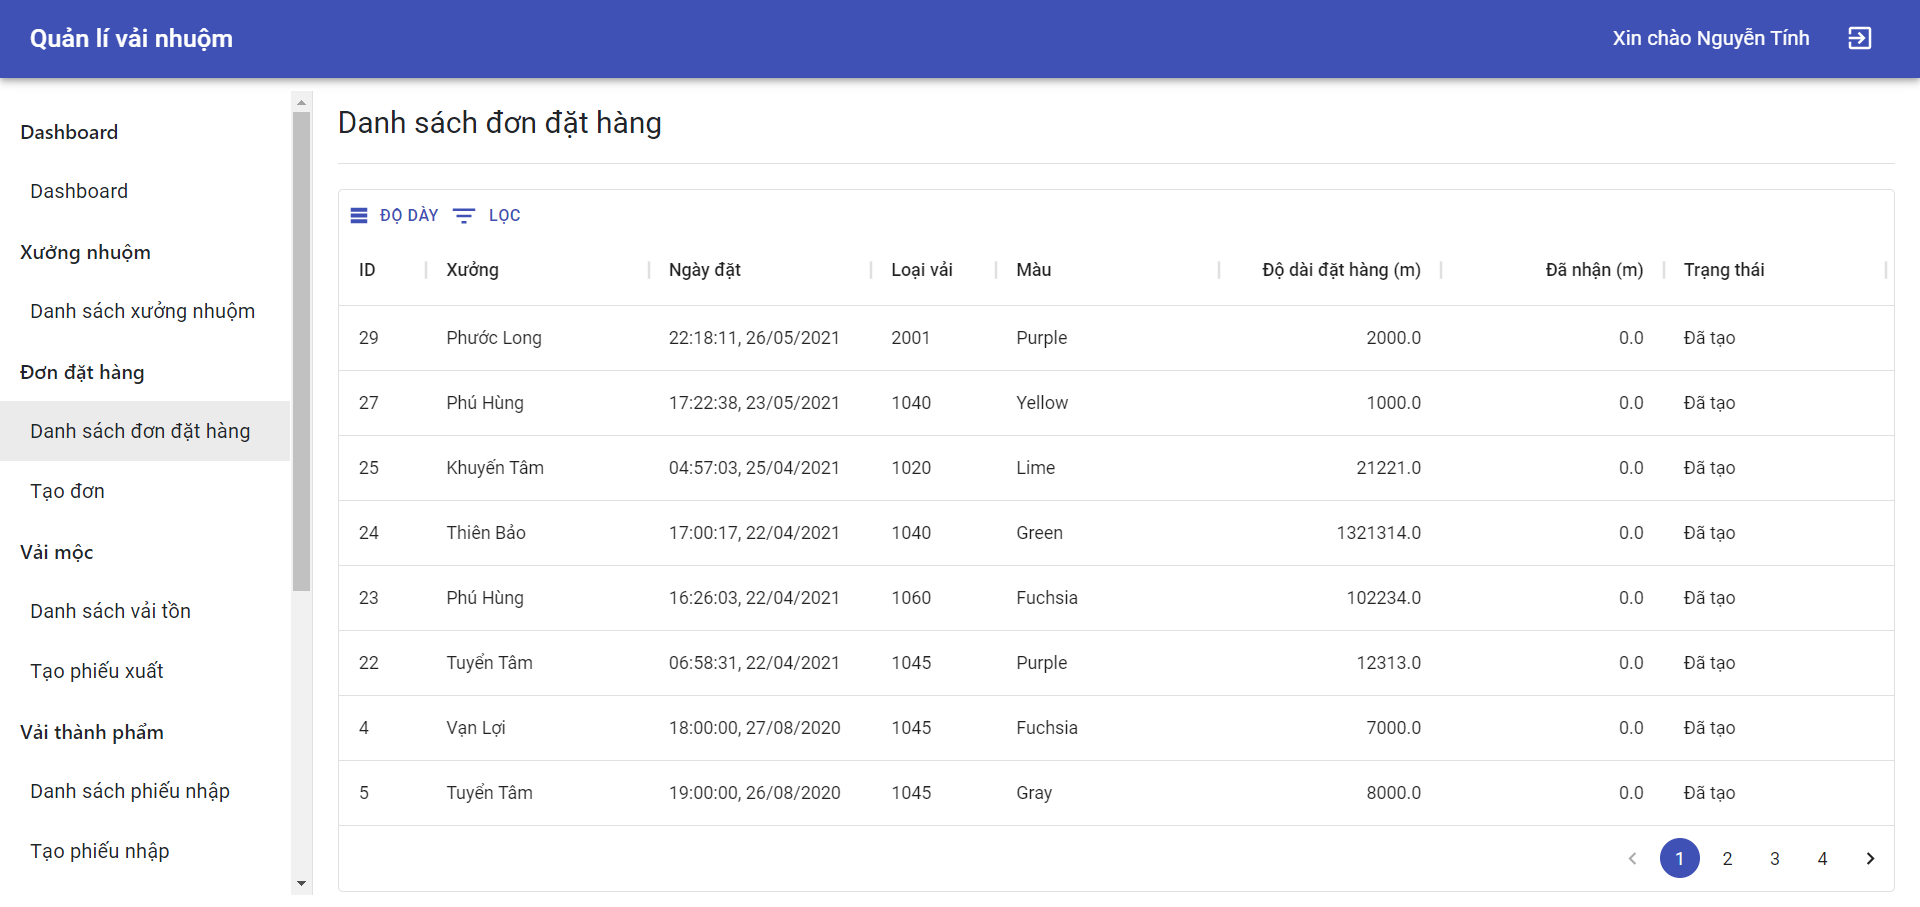
\includegraphics[width=14cm]{Image/result/danh_sach_don_hang.png}}
        \caption{Giao diện trang Danh sách đơn đặt hàng}
        \label{result_danh_sach_don_hang}
    \end{center}
\end{figure}

Ở trang Chi tiết đơn đặt hàng, nhân viên còn có thể cập nhật trạng thái đơn hàng Hủy đơn hàng (áp dụng cho các đơn hàng có trạng thái mới tạo), Hoàn thành đơn hàng (áp dụng cho các đơn hàng ở trạng thái đang xử lí). \par

\begin{figure}[H]
    \begin{center}
        \frame{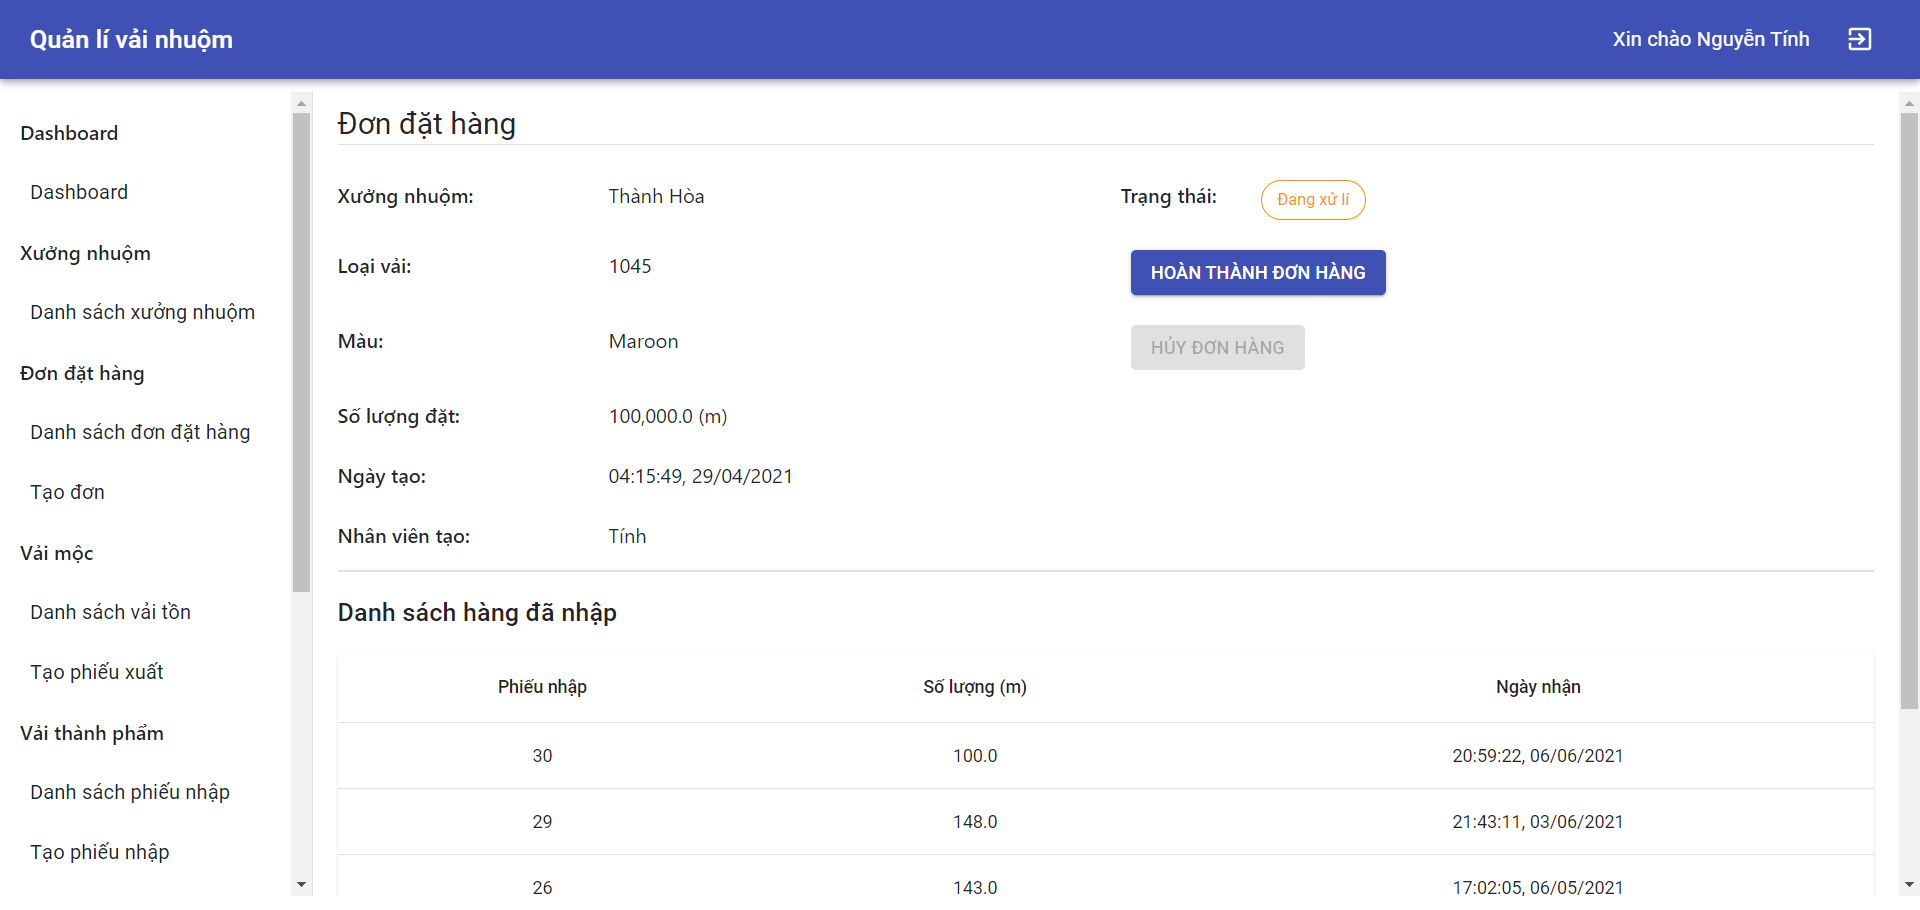
\includegraphics[width=14cm]{Image/result/chi_tiet_don_hang.png}}
        \caption{Giao diện trang Chi tiết đơn đặt hàng}
        \label{result_chi_tiet_don_hang}
    \end{center}
\end{figure}

\begin{figure}[H]
    \begin{center}
        \frame{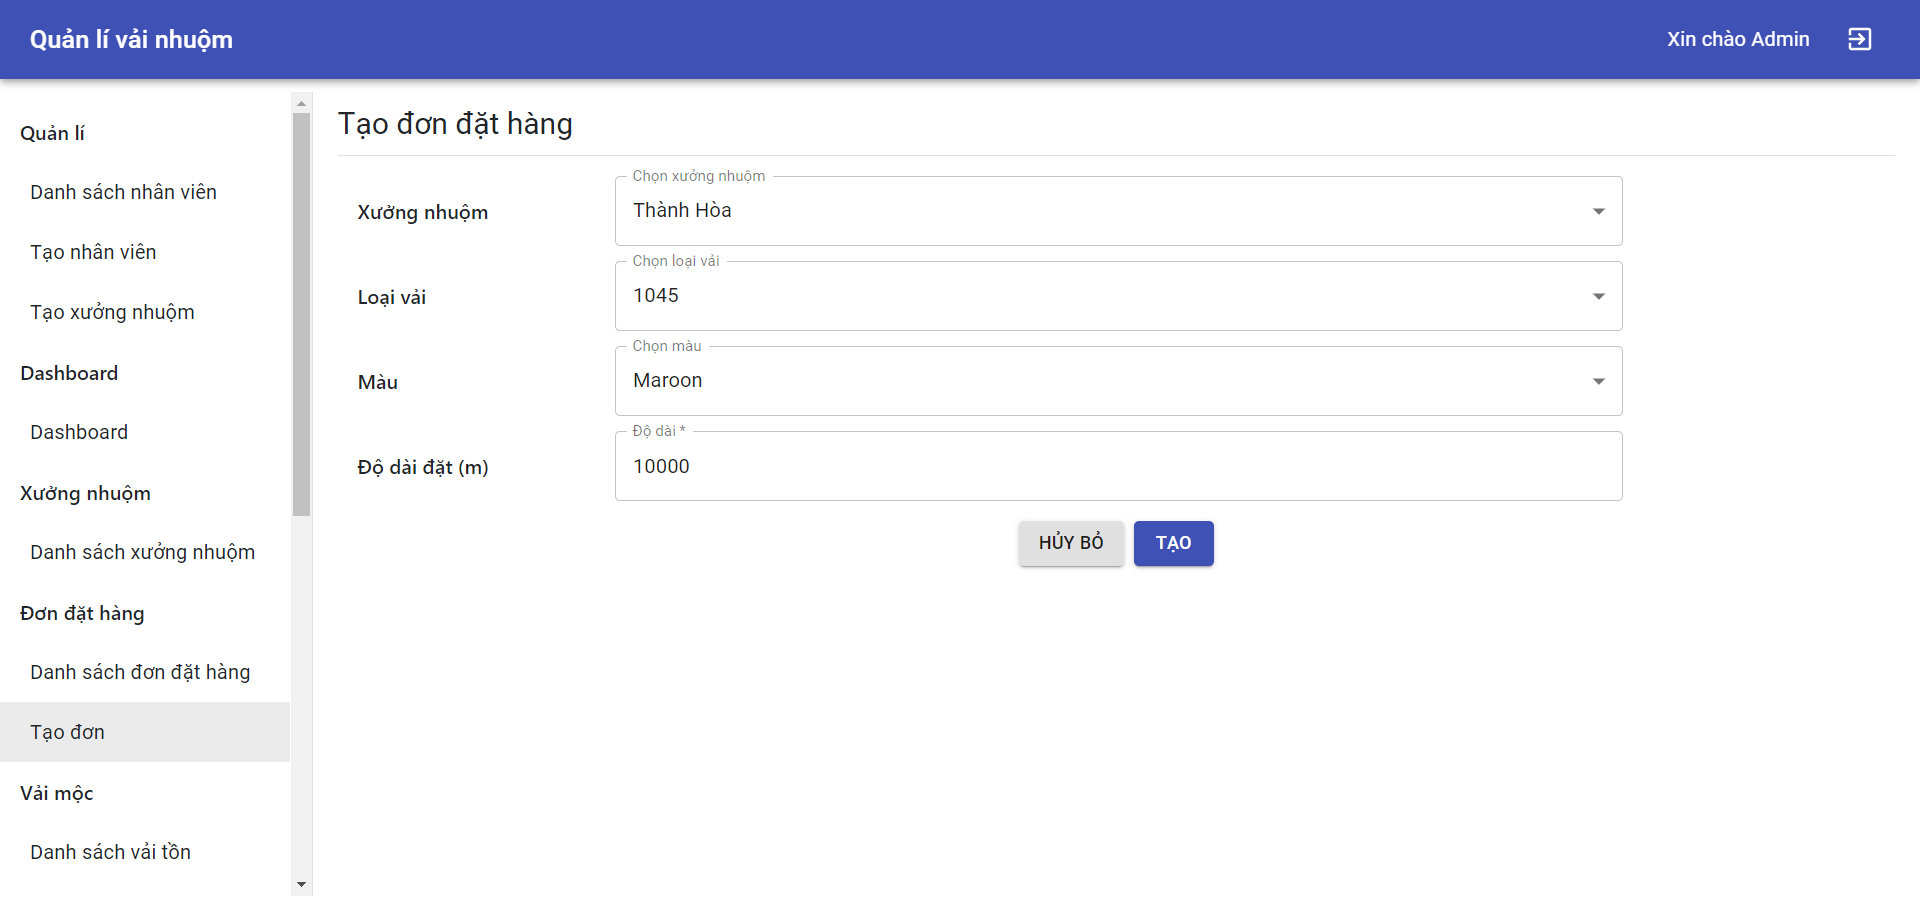
\includegraphics[width=14cm]{Image/result/tao_don_hang.png}}
        \caption{Giao diện trang Tạo đơn đặt hàng}
        \label{result_tao_don_hang}
    \end{center}
\end{figure}

%%%%%%%%%%%%%%%%%%%%%%%%
\textbf{Quản lí vải mộc}

Ở nhóm chức năng này, người dùng có thể xem thống kê số lượng vải mộc đang còn tồn kho ở công ty [Hình \ref{result_moc_ton_kho}], tồn kho ở xưởng [Hình \ref{result_ton_kho_xuong}], và tạo một phiếu xuất vải mộc mới cho xưởng [Hình \ref{result_tao_phieu_xuat}].

\begin{figure}[H]
    \begin{center}
        \frame{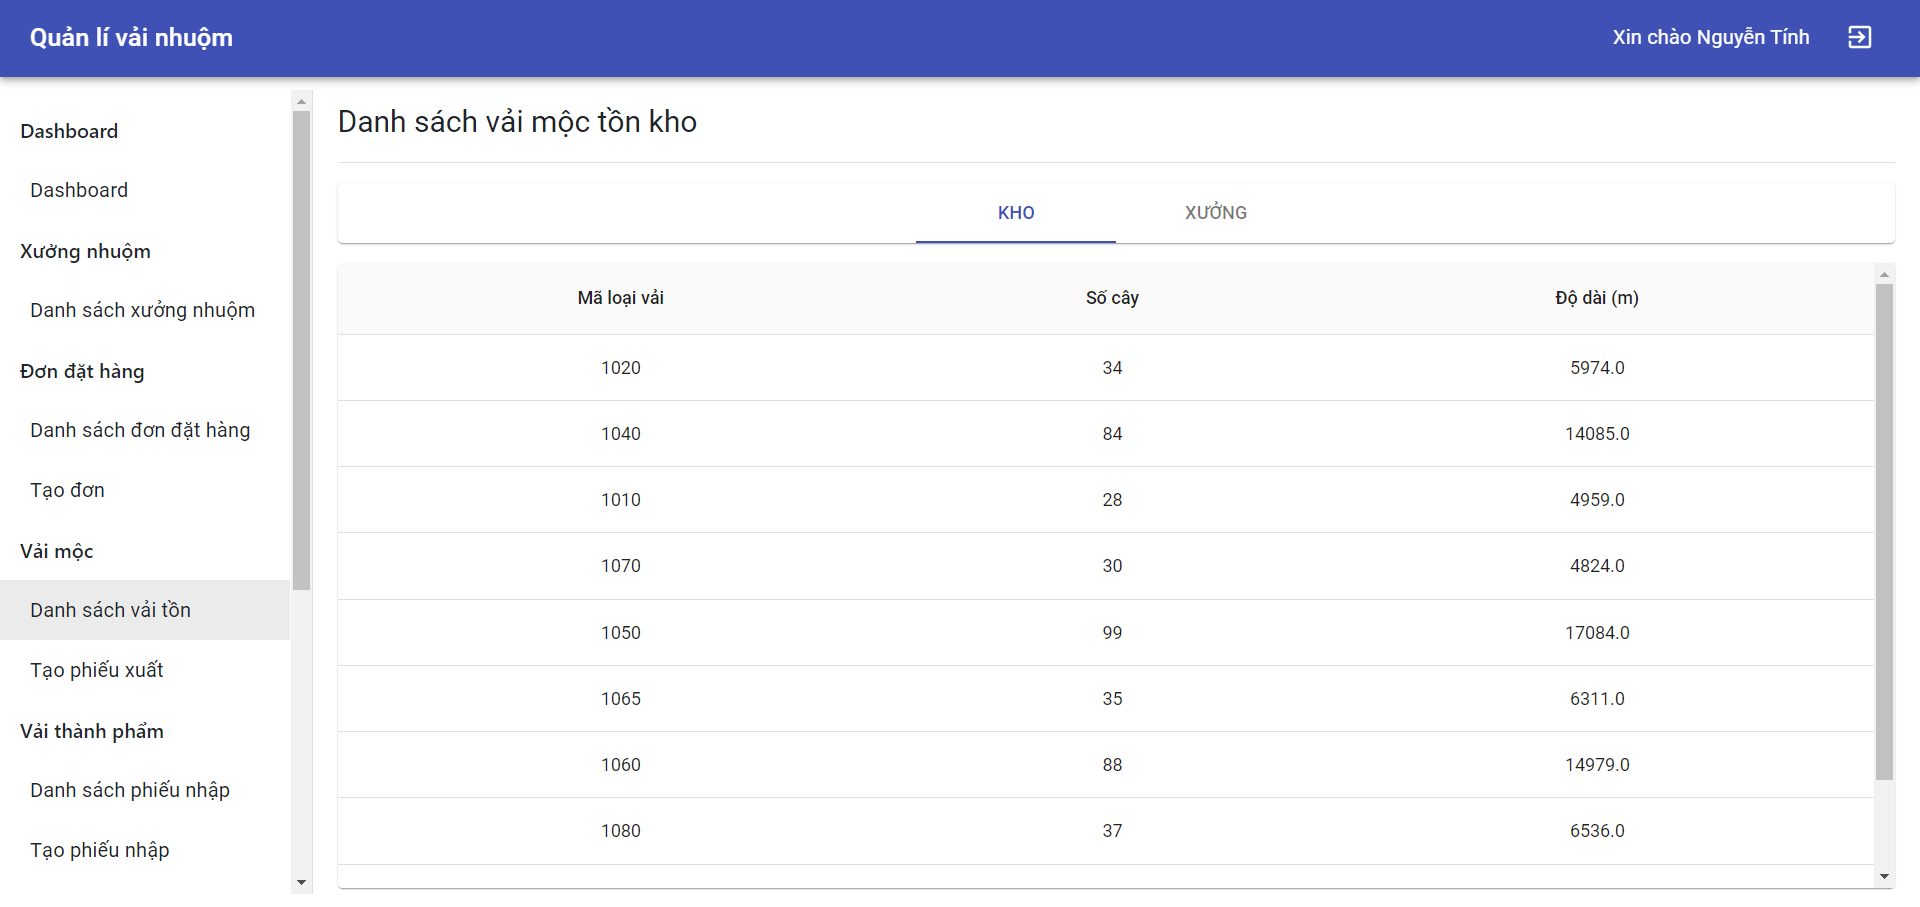
\includegraphics[width=14cm]{Image/result/moc_ton_kho.png}}
        \caption{Giao diện trang Vải mộc tồn ở kho}
        \label{result_moc_ton_kho}
    \end{center}
\end{figure}

\begin{figure}[H]
    \begin{center}
        \frame{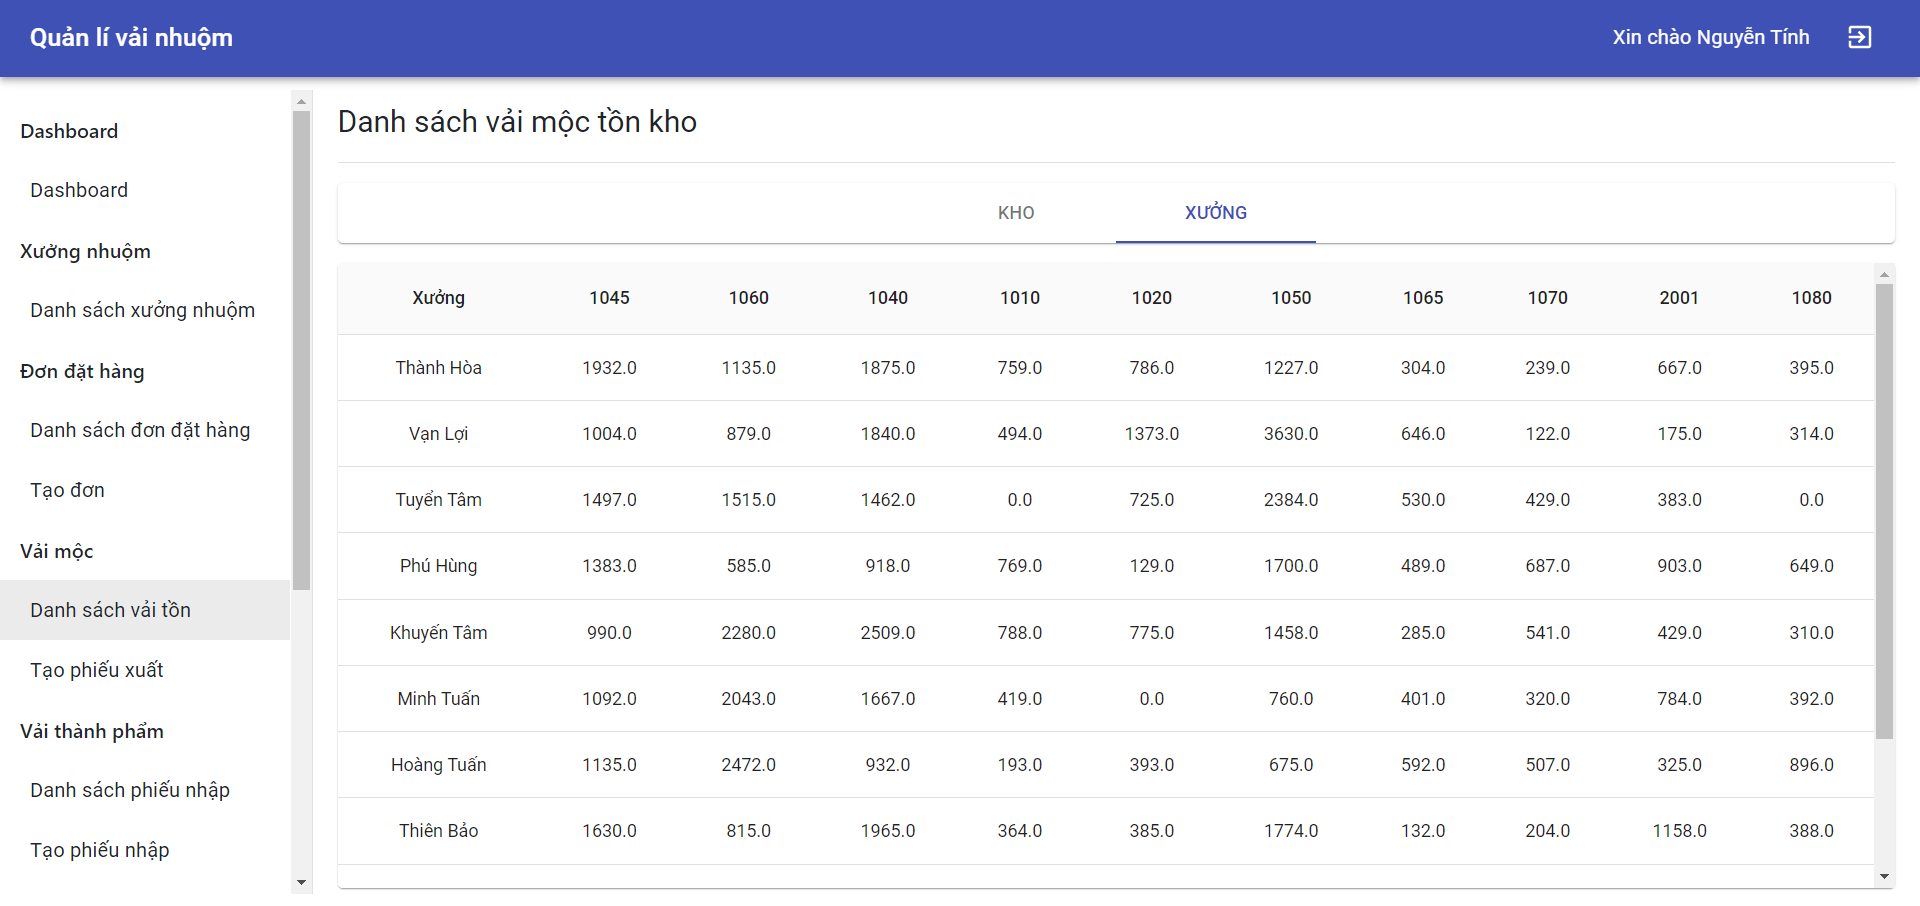
\includegraphics[width=14cm]{Image/result/moc_ton_xuong.png}}
        \caption{Giao diện trang Vải mộc tồn ở xưởng}
        \label{result_moc_ton_xuong}
    \end{center}
\end{figure}

\begin{figure}[H]
    \begin{center}
        \frame{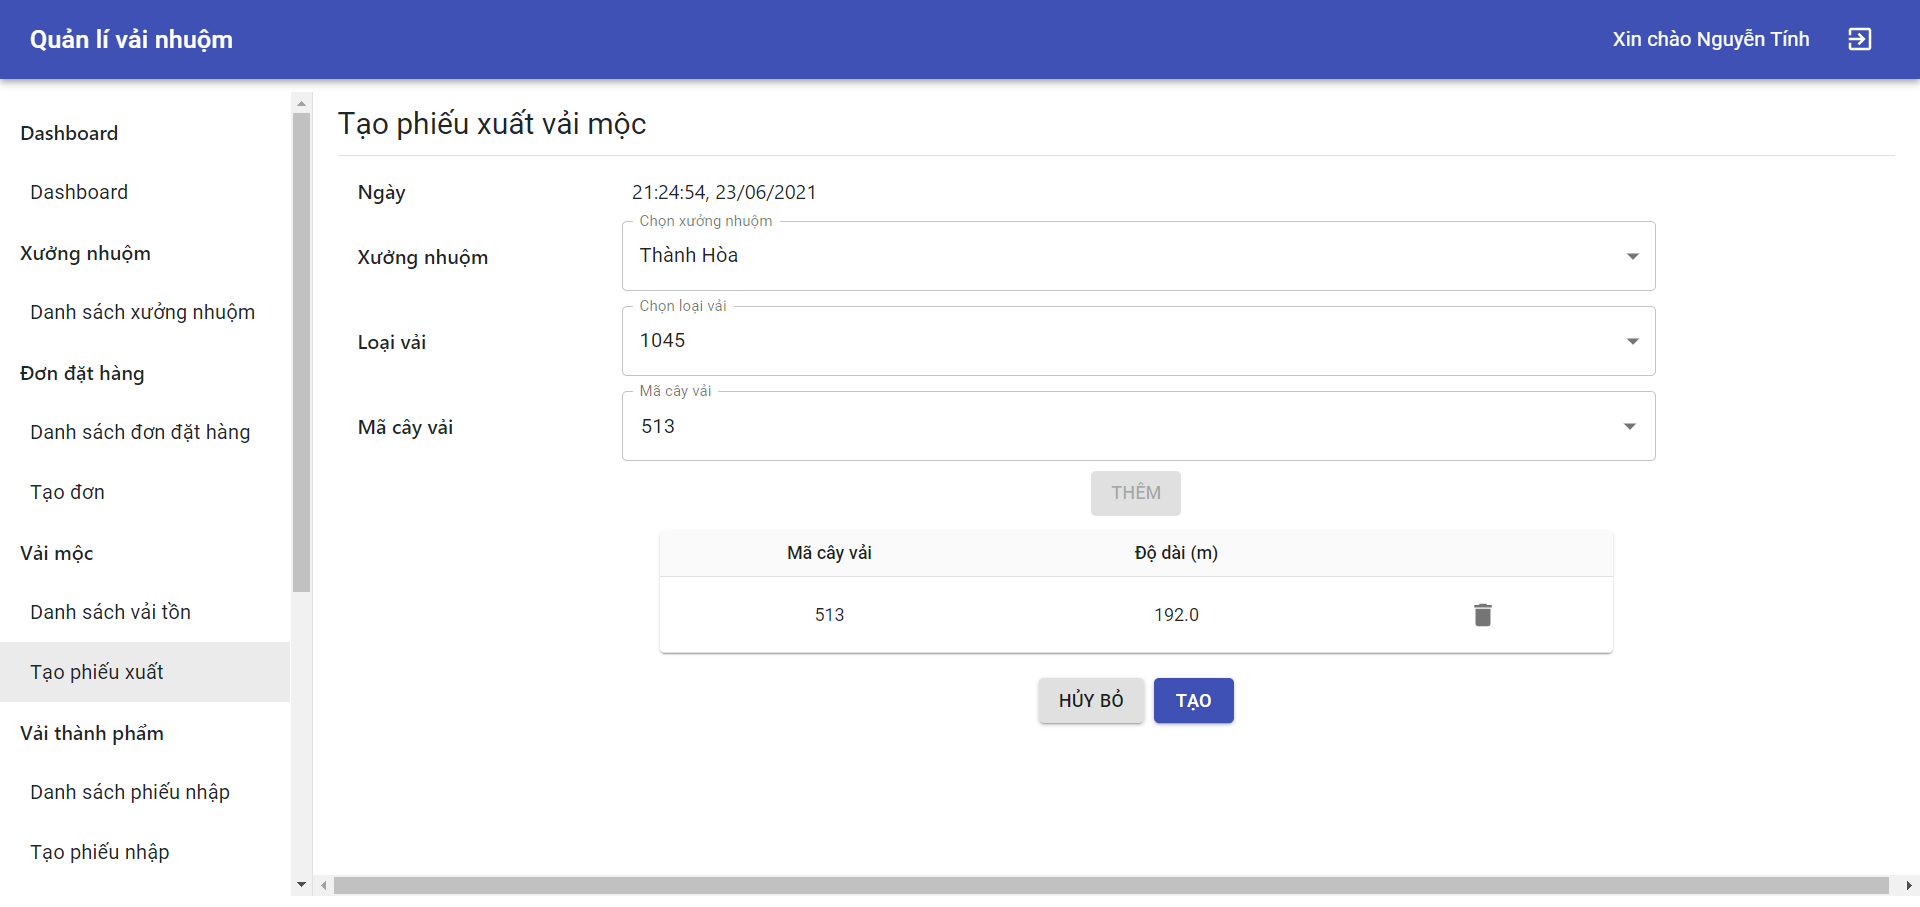
\includegraphics[width=14cm]{Image/result/tao_phieu_xuat.png}}
        \caption{Giao diện trang Tạo phiếu xuất vải mộc}
        \label{result_tao_phieu_xuat}
    \end{center}
\end{figure}

%%%%%%%%%%%%%%%%%%%%%%%%
\textbf{Quản lí vải thành phẩm}

Ở nhóm chức năng này, người dùng có thể xem danh sách các phiếu nhập hàng thành phẩm về công ty [Hình \ref{result_danh_sach_phieu_nhap}], thông tin chi tiết về một phiếu gồm có danh sách chi tiết từng cây vải [Hình \ref{result_chi_tiet_phieu_nhap}], và tạo một phiếu nhập mới [Hình \ref{result_tao_phieu_nhap_1} \& \ref{result_tao_phieu_nhap_2}].

\begin{figure}[H]
    \begin{center}
        \frame{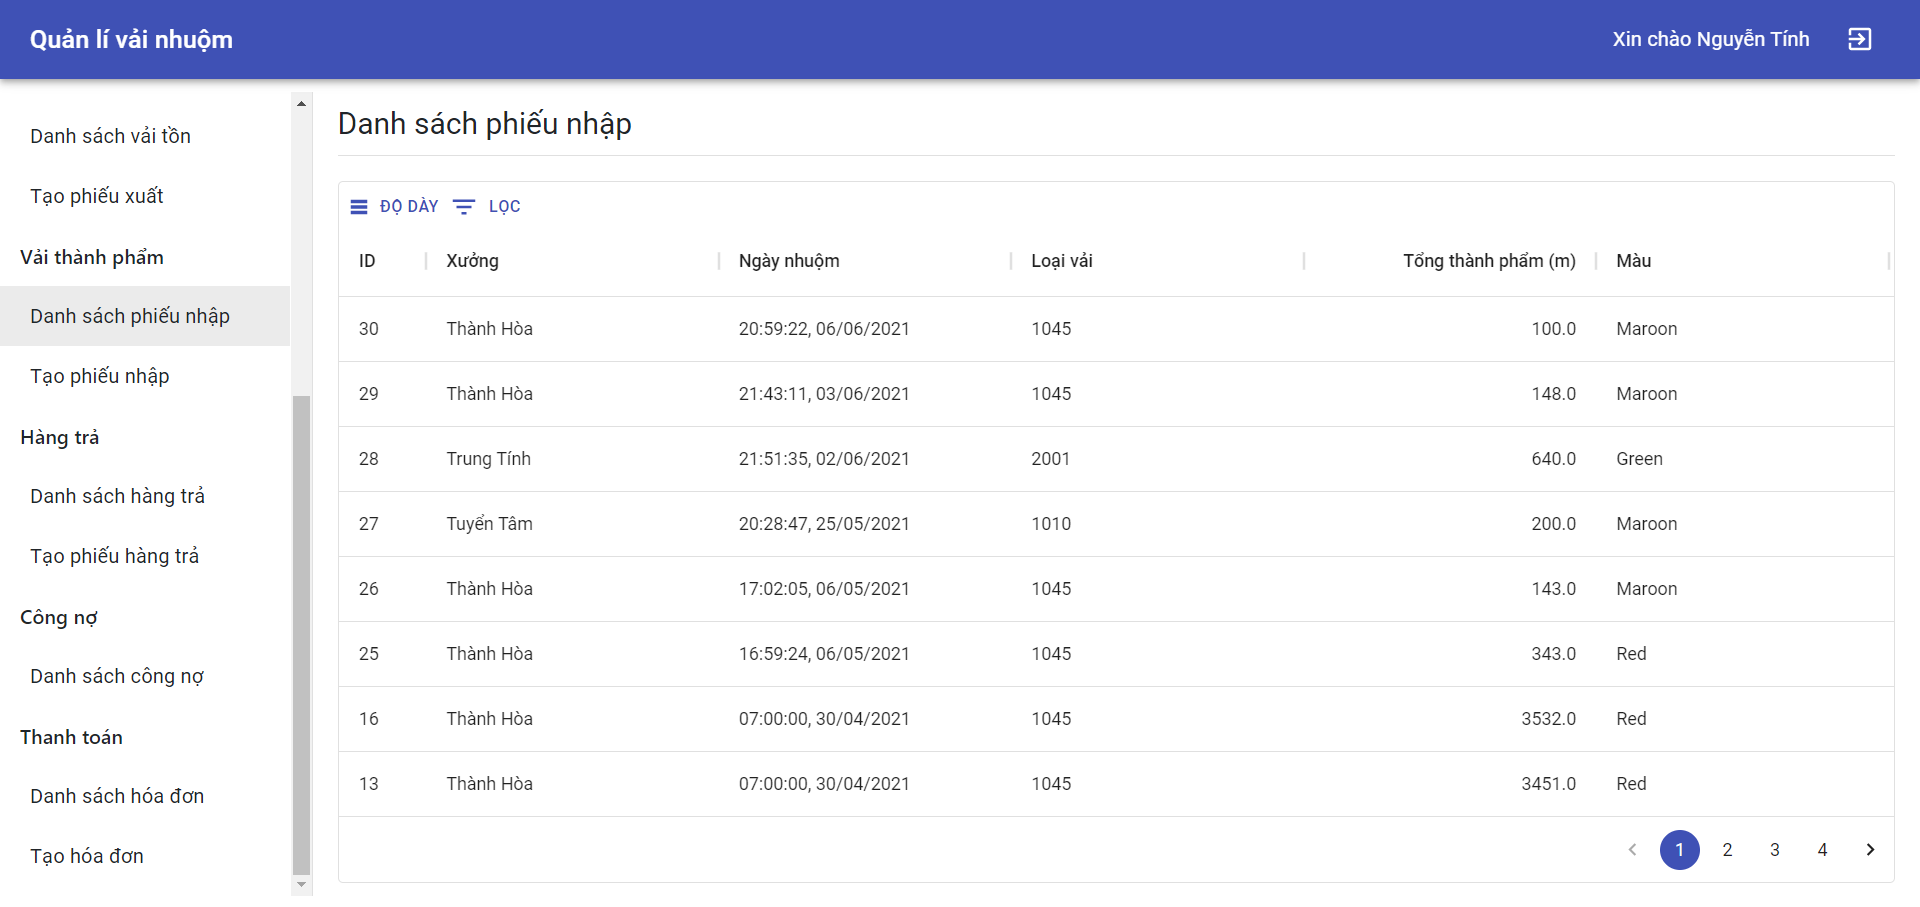
\includegraphics[width=14cm]{Image/result/danh_sach_phieu_nhap.png}}
        \caption{Giao diện trang Danh sách phiếu nhập}
        \label{result_danh_sach_phieu_nhap}
    \end{center}
\end{figure}

\begin{figure}[H]
    \begin{center}
        \frame{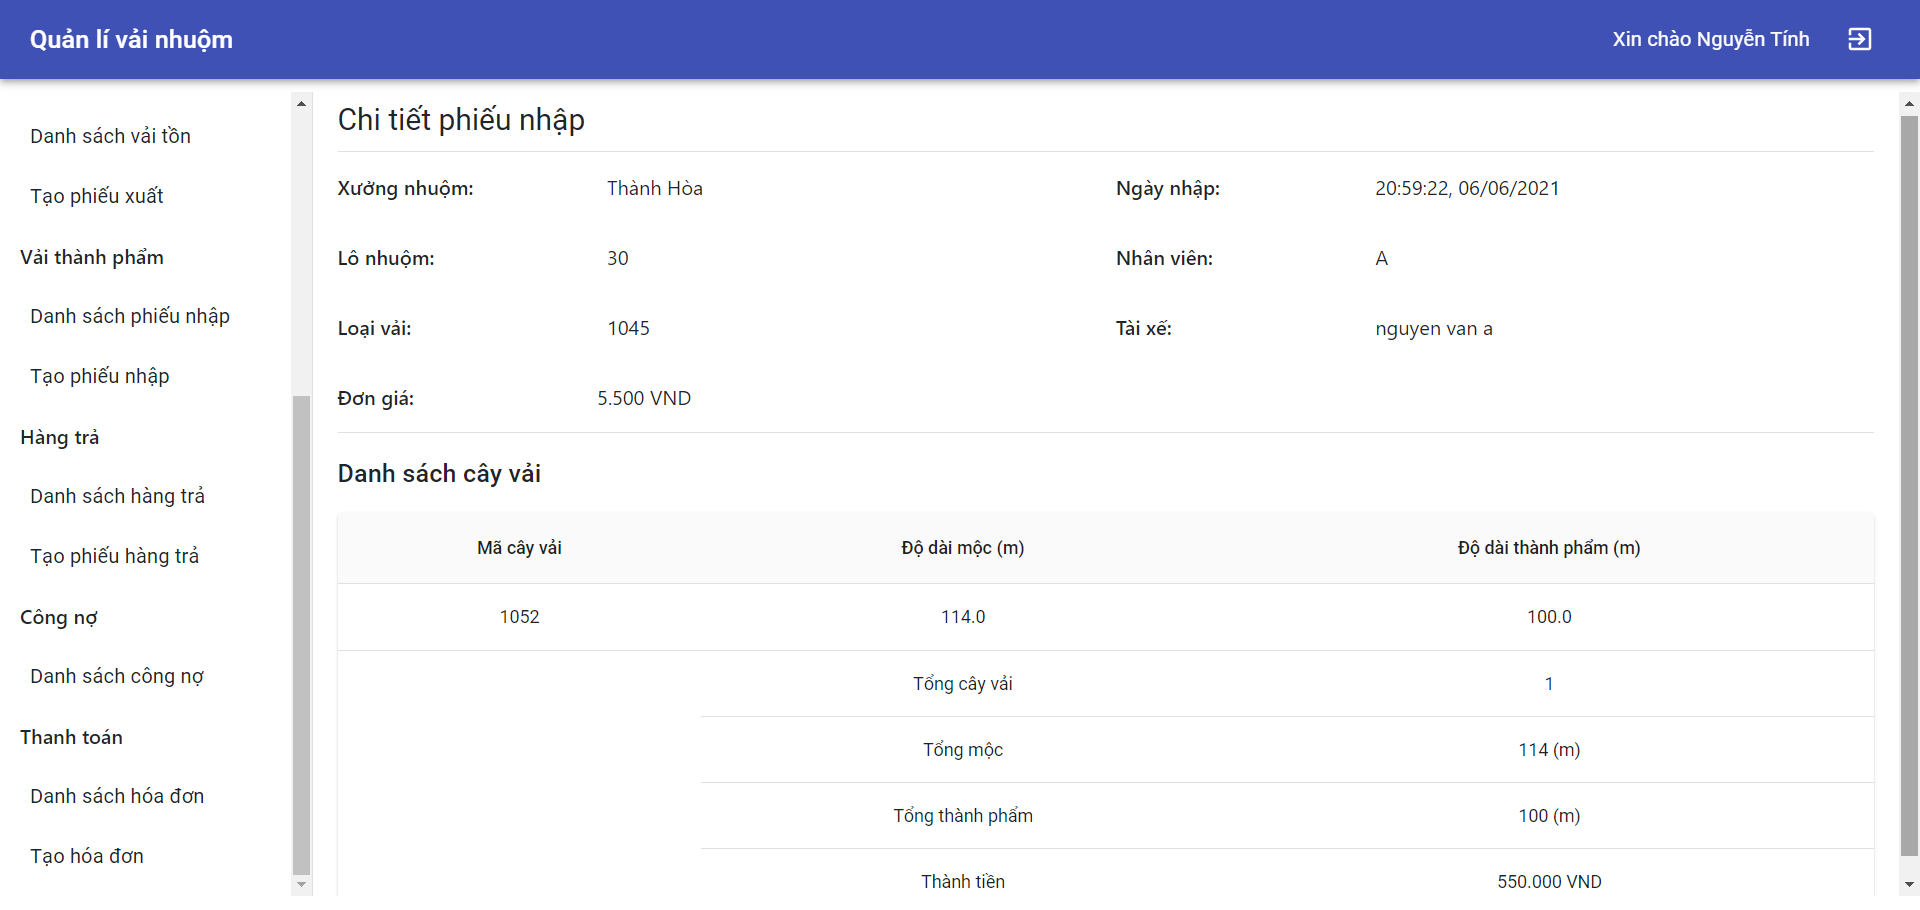
\includegraphics[width=14cm]{Image/result/chi_tiet_phieu_nhap.png}}
        \caption{Giao diện trang Chi tiết phiếu nhập}
        \label{result_chi_tiet_phieu_nhap}
    \end{center}
\end{figure}

Ở trang Tạo phiếu nhập, danh sách đơn đặt hàng người dùng có thể chọn chính là các đơn đặt hàng thỏa mãn ba thông tin phía trên gồm xưởng nhuộm, loại vải, màu nhuộm. Danh sách các cây vải chính là những cây vải thỏa mãn hai thông tin gồm xưởng nhuộm và loại vải. \par

\begin{figure}[H]
    \begin{center}
        \frame{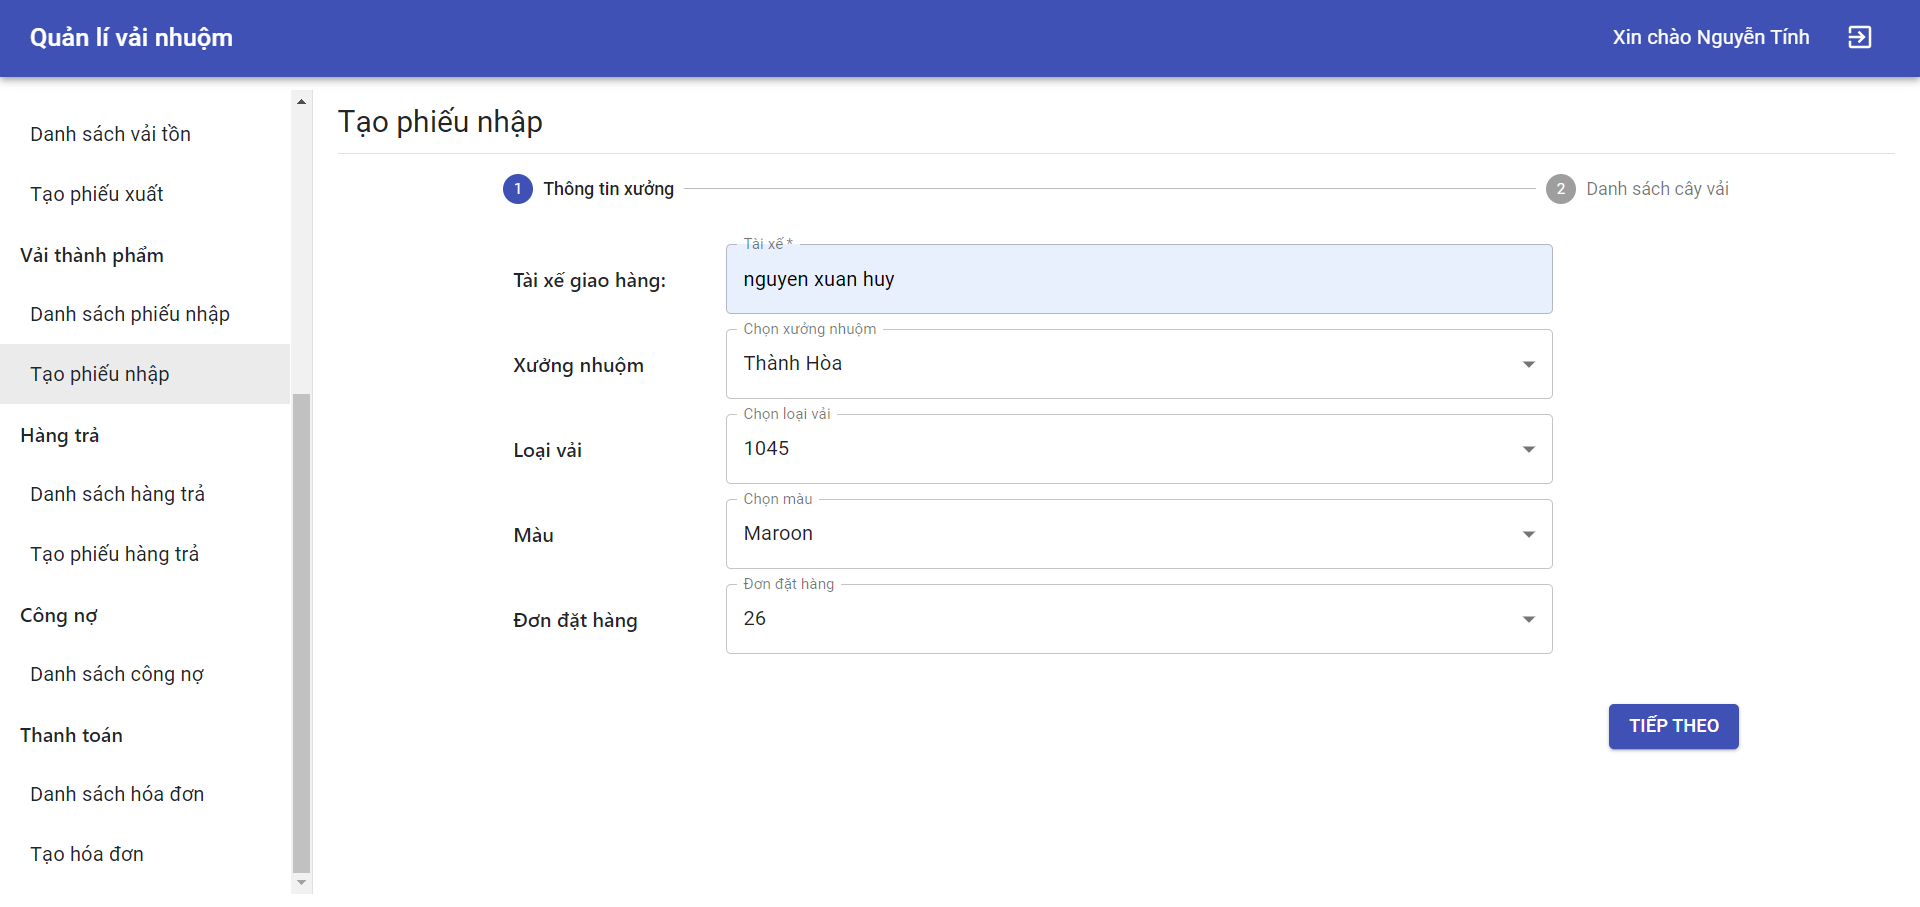
\includegraphics[width=14cm]{Image/result/tao_phieu_nhap_1.png}}
        \caption{Giao diện trang Tạo phiếu nhập - 1}
        \label{result_tao_phieu_nhap_1}
    \end{center}
\end{figure}

\begin{figure}[H]
    \begin{center}
        \frame{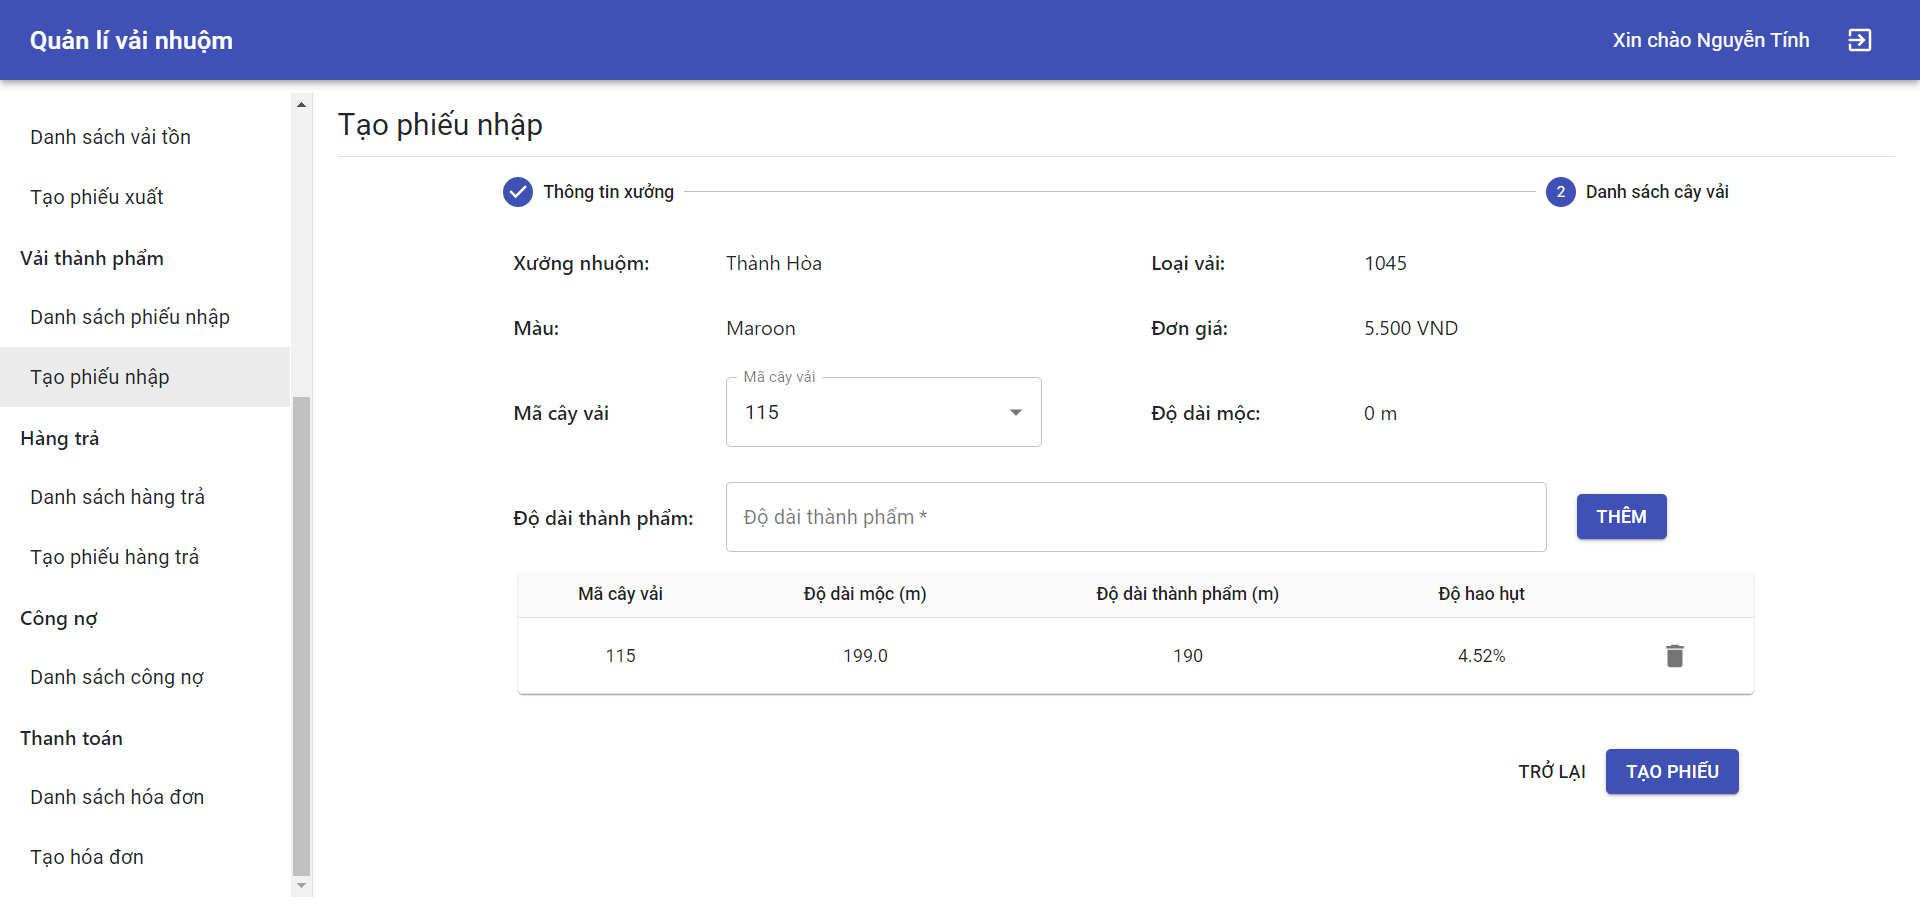
\includegraphics[width=14cm]{Image/result/tao_phieu_nhap_2.png}}
        \caption{Giao diện trang Tạo phiếu nhập - 2}
        \label{result_tao_phieu_nhap_2}
    \end{center}
\end{figure}

%%%%%%%%%%%%%%%%%%%%%%%%
\textbf{Quản lí hàng trả}

Ở nhóm chức năng này, người dùng có thể xem danh sách các phiếu hàng trả cho xưởng [Hình \ref{result_danh_sach_hang_tra}], xem chi tiết phiếu hàng trả bao gồm các cây vải và lí do trả [Hình \ref{result_chi_tiet_hang_tra}], và tạo một phiếu hàng trả mới [Hình \ref{result_tao_hang_tra}].

\begin{figure}[H]
    \begin{center}
        \frame{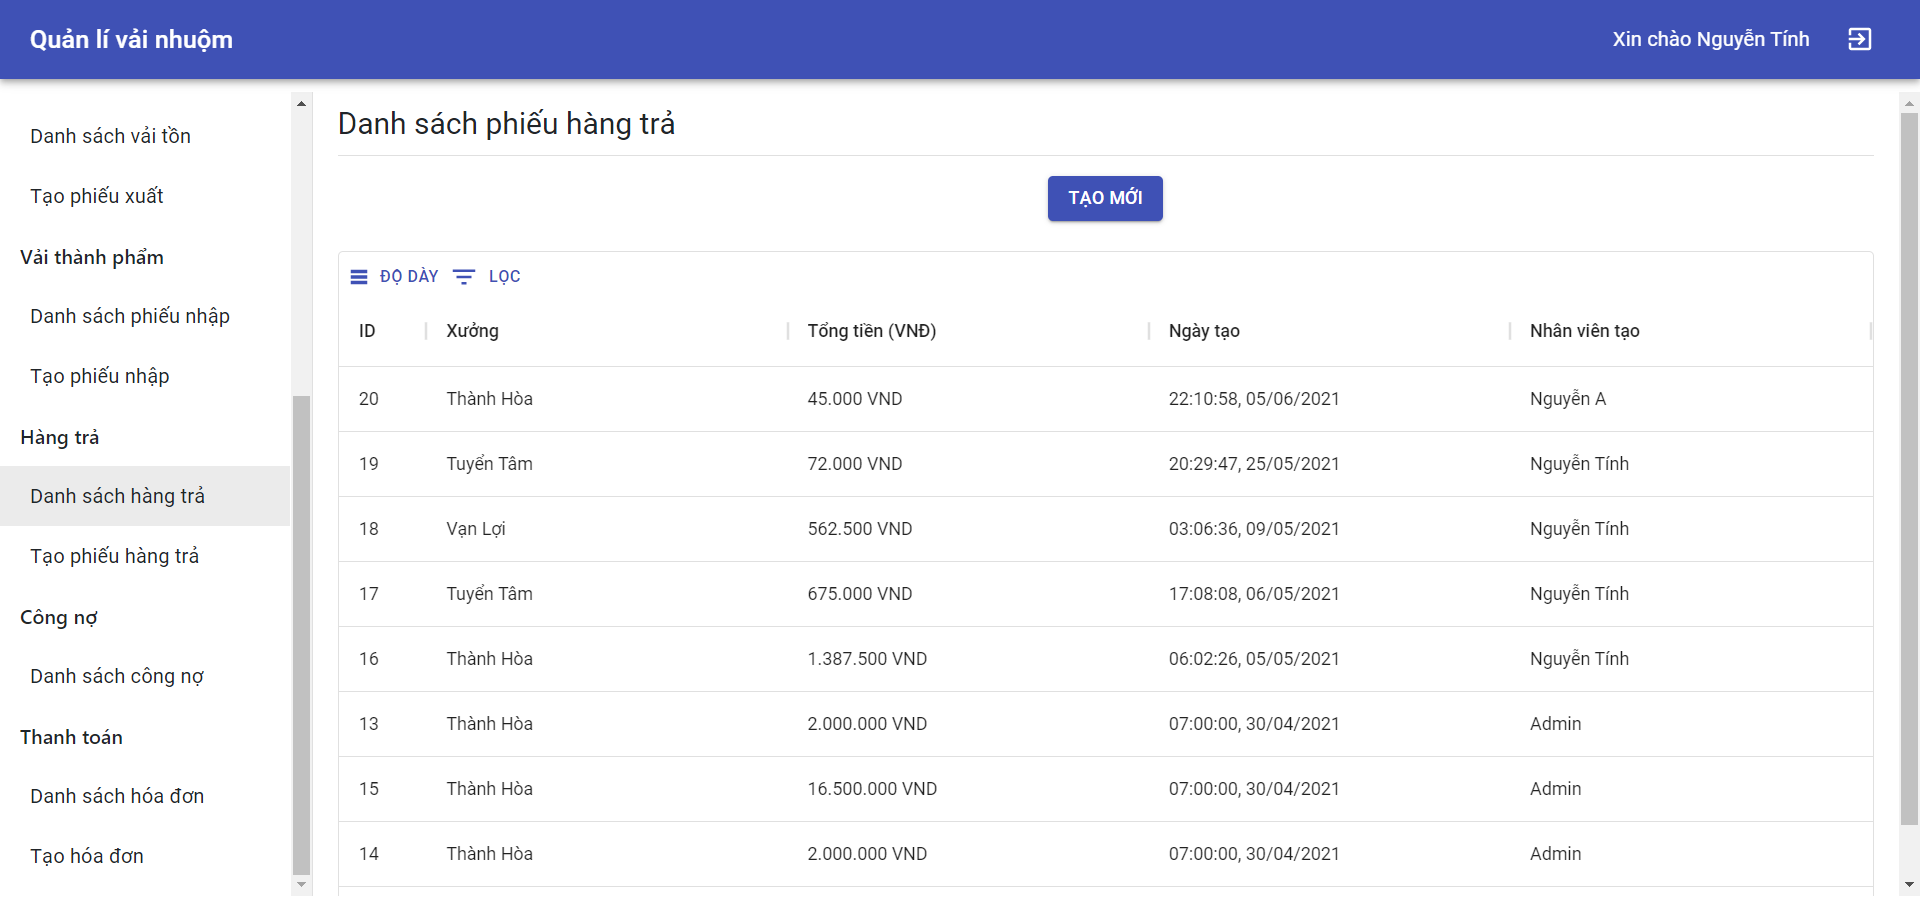
\includegraphics[width=14cm]{Image/result/danh_sach_hang_tra.png}}
        \caption{Giao diện trang Danh sách phiếu hàng trả}
        \label{result_danh_sach_hang_tra}
    \end{center}
\end{figure}

\begin{figure}[H]
    \begin{center}
        \frame{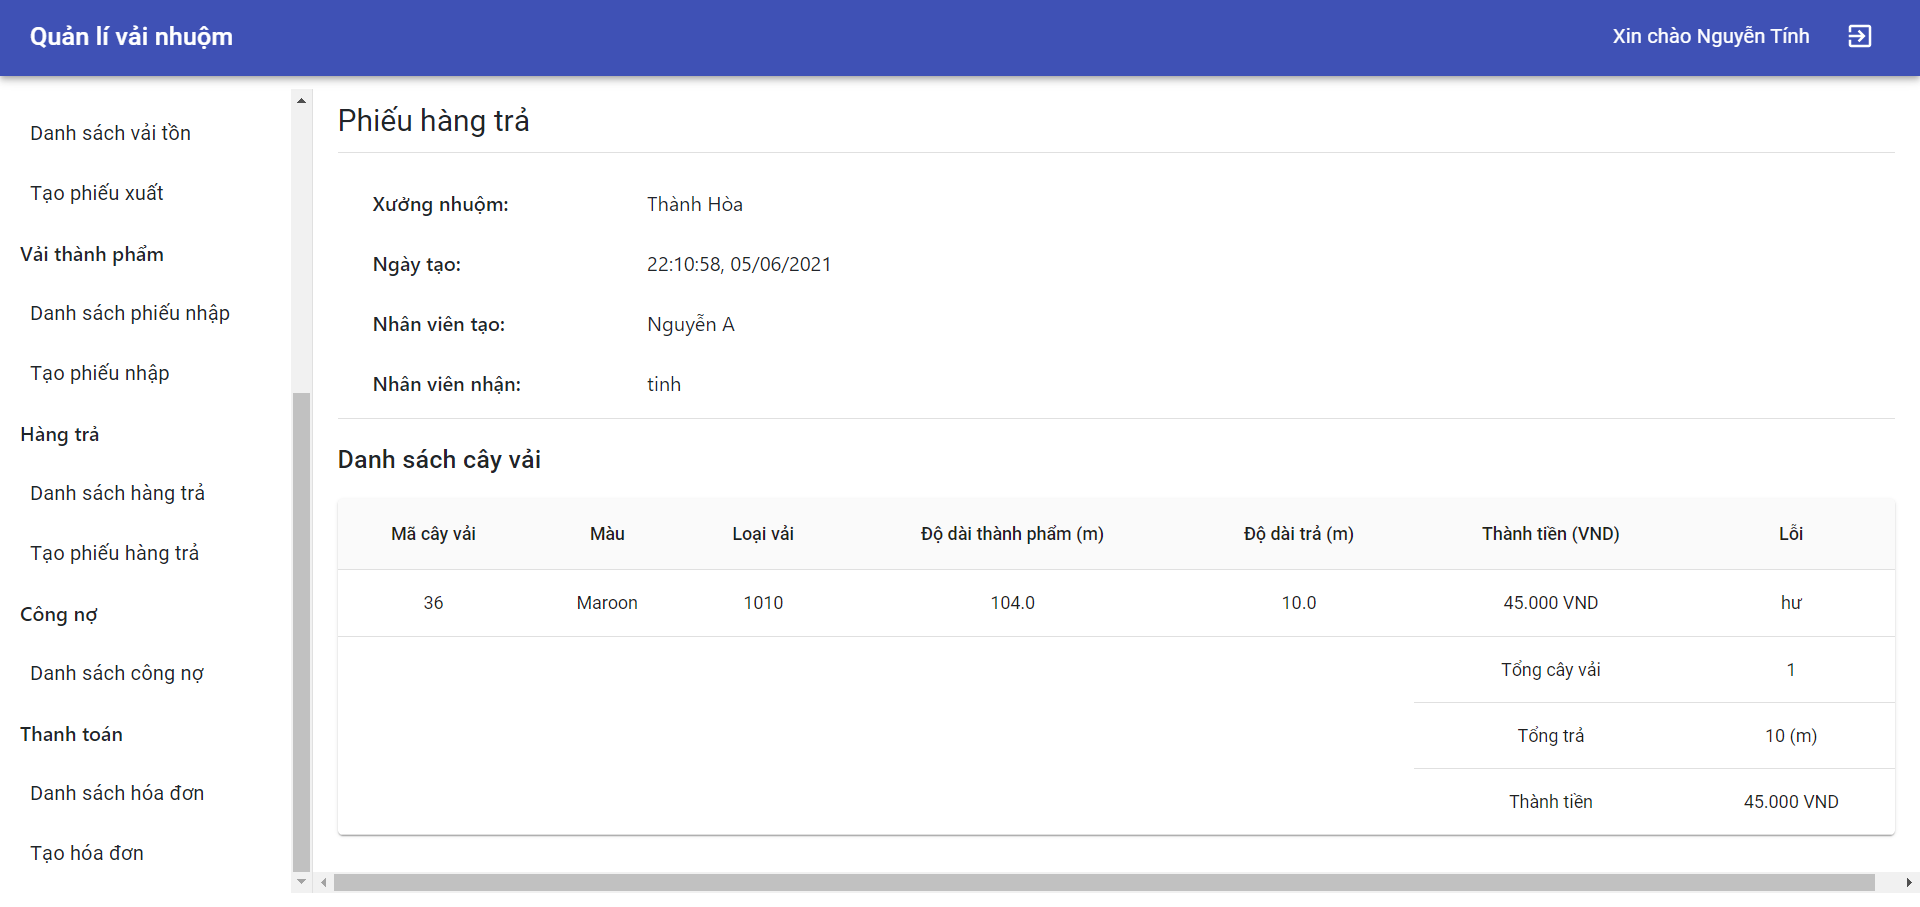
\includegraphics[width=14cm]{Image/result/chi_tiet_hang_tra.png}}
        \caption{Giao diện trang Chi tiết phiếu hàng trả}
        \label{result_chi_tiet_hang_tra}
    \end{center}
\end{figure}

Ở trang Tạo phiếu hàng trả, danh sách mã cây vải là những cây vải thành phẩm đã được nhuộm ở xưởng nhuộm đã chọn. \par

\begin{figure}[H]
    \begin{center}
        \frame{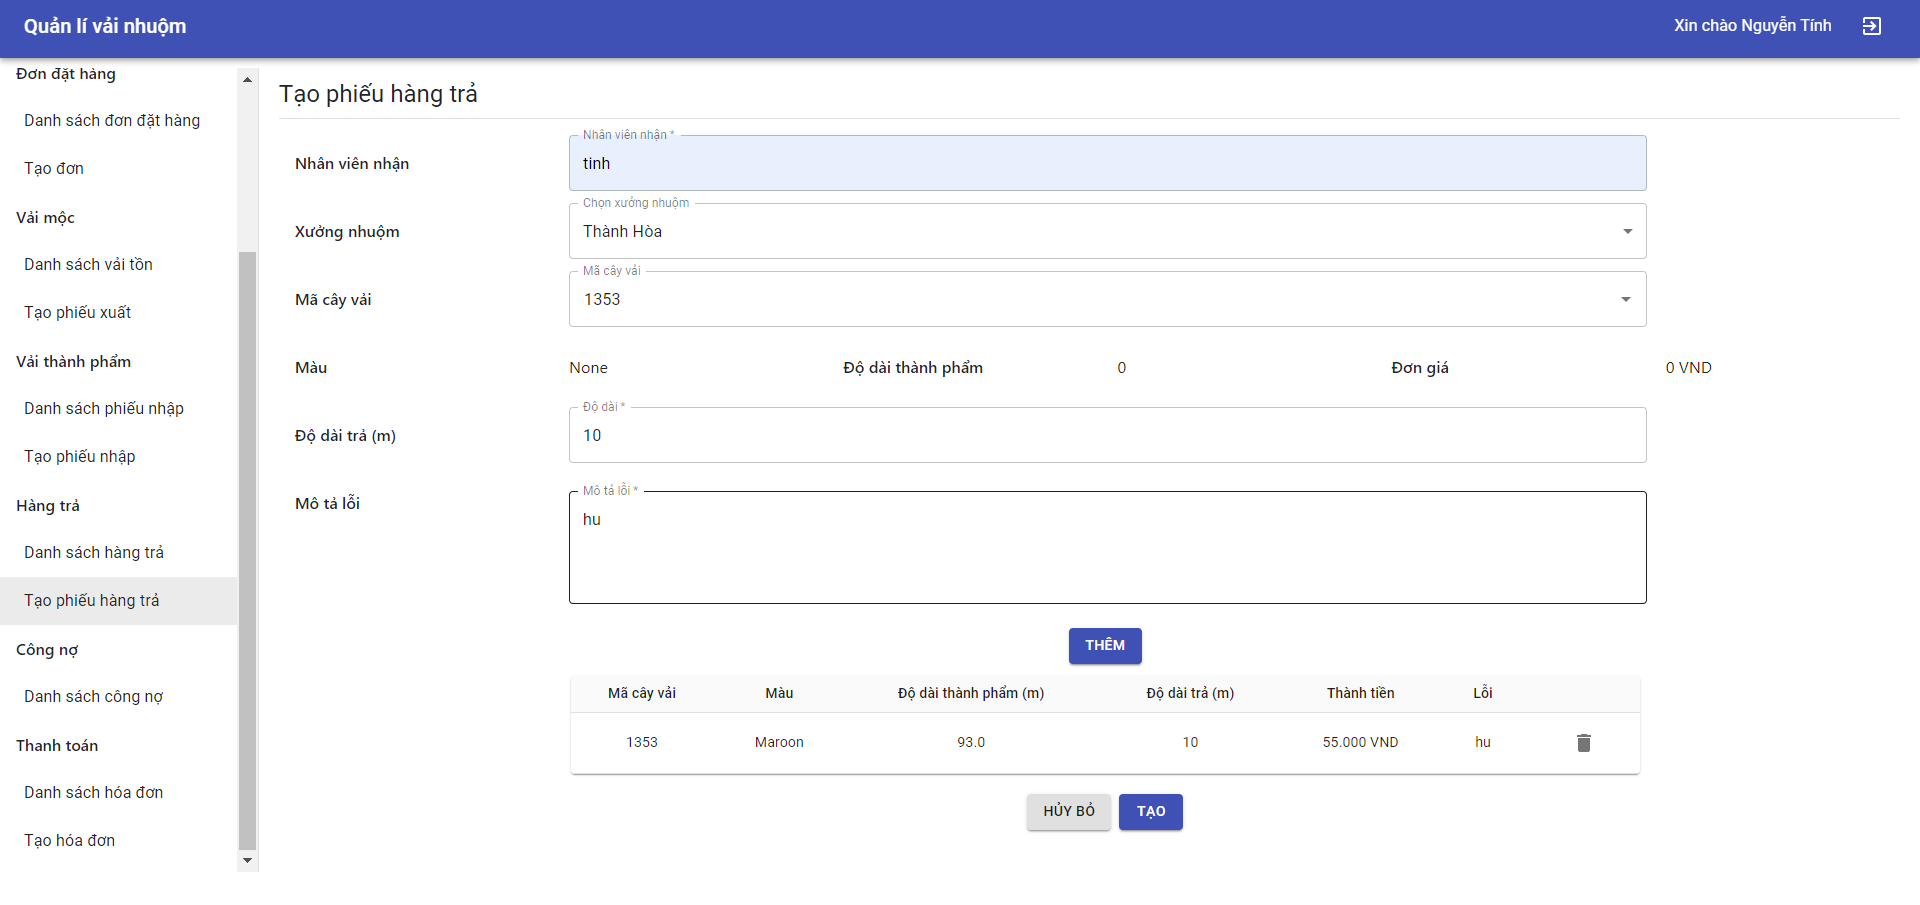
\includegraphics[width=14cm]{Image/result/tao_hang_tra.png}}
        \caption{Giao diện trang Tạo phiếu hàng trả}
        \label{result_tao_hang_tra}
    \end{center}
\end{figure}

%%%%%%%%%%%%%%%%%%%%%%%%
\textbf{Quản lí công nợ}

Ở nhóm chức năng này, người dùng có thể xem danh sách công nợ của các xưởng [Hình \ref{result_danh_sach_cong_no}], thông tin chi tiết các giao dịch công nợ của xưởng [Hình \ref{result_chi_tiet_cong_no}], danh sách các hóa đơn thanh toán cho các xưởng [Hình \ref{result_danh_sach_hoa_don_thanh_toan}], và tạo một hóa đơn thanh toán mới [Hình \ref{result_tao_hoa_don_thanh_toan}].

\begin{figure}[H]
    \begin{center}
        \frame{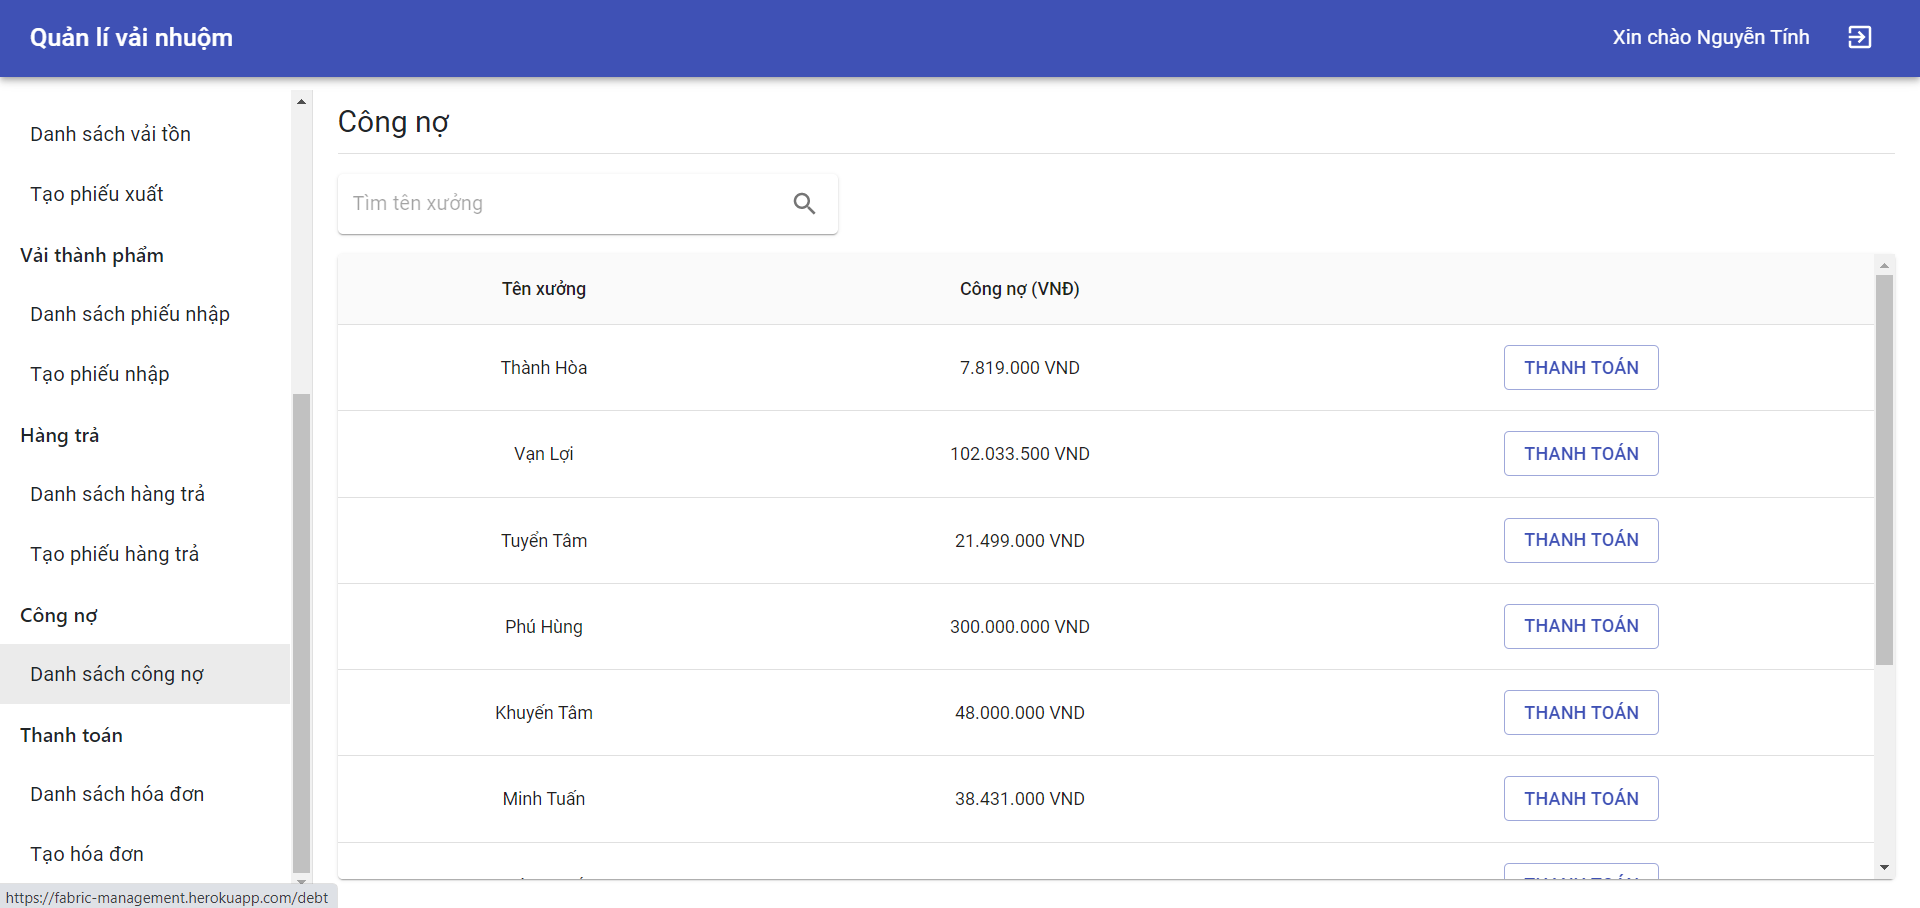
\includegraphics[width=14cm]{Image/result/danh_sach_cong_no.png}}
        \caption{Giao diện trang Danh sách công nợ}
        \label{result_danh_sach_cong_no}
    \end{center}
\end{figure}

\begin{figure}[H]
    \begin{center}
        \frame{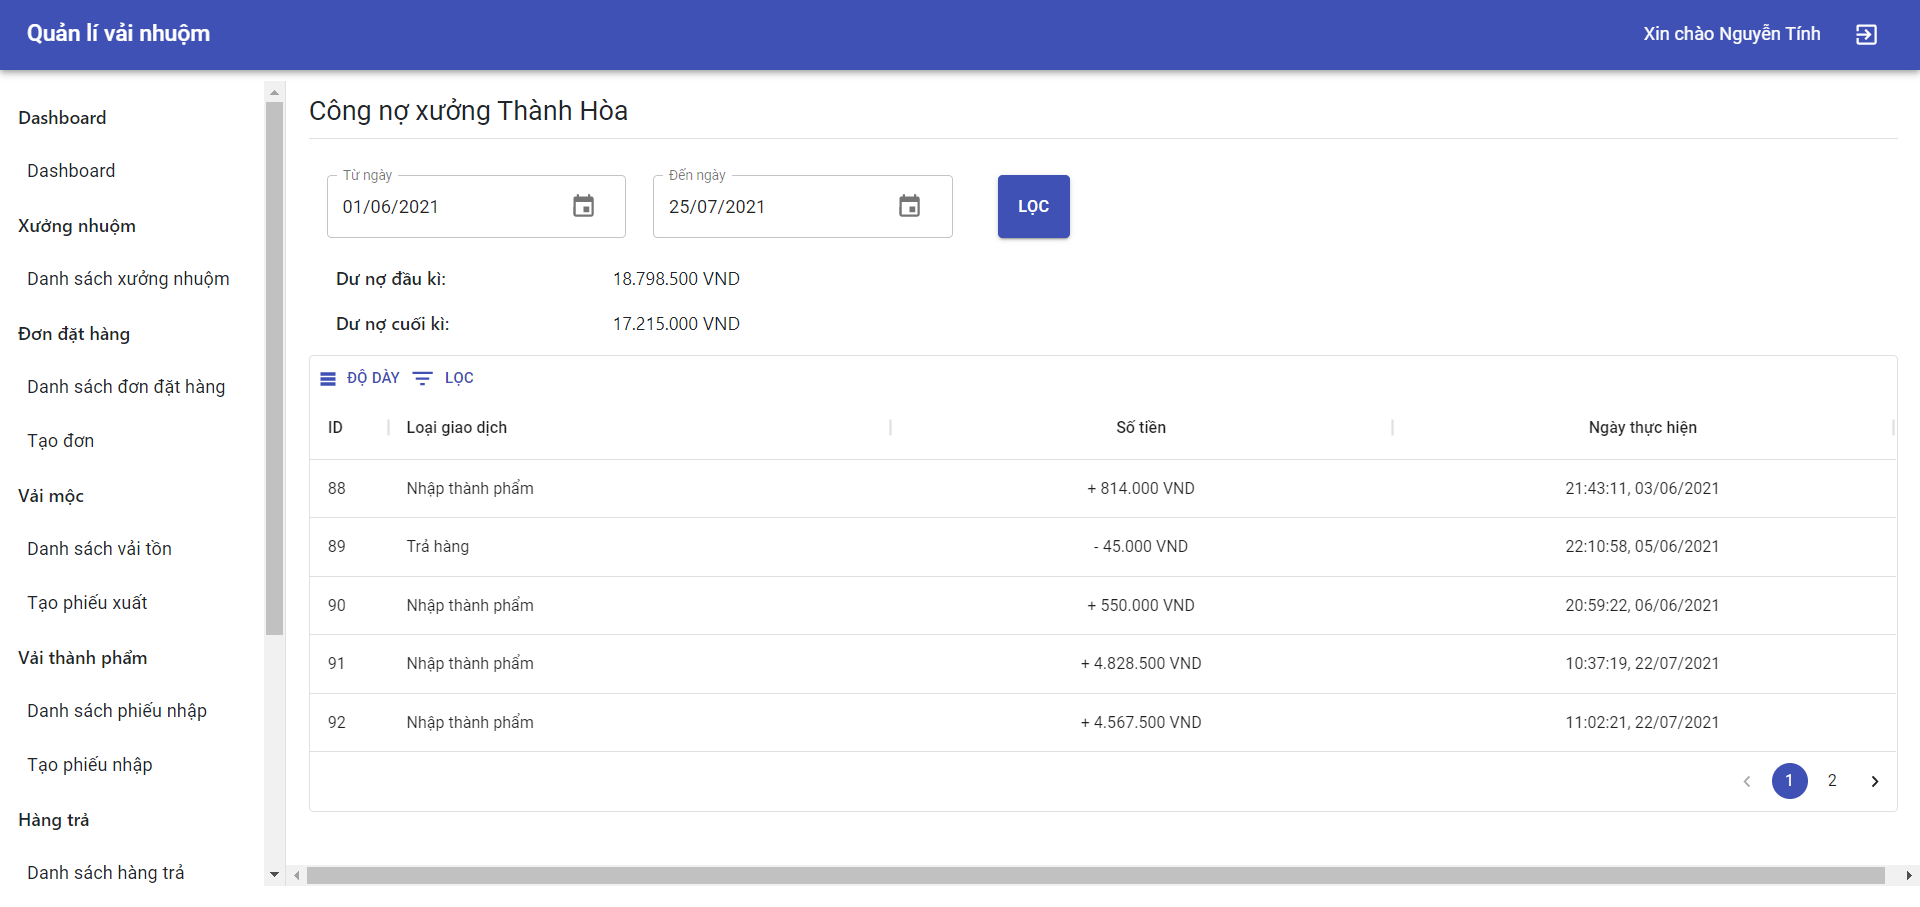
\includegraphics[width=14cm]{Image/result/chi_tiet_cong_no.png}}
        \caption{Giao diện trang Chi tiết công nợ}
        \label{result_chi_tiet_cong_no}
    \end{center}
\end{figure}

\begin{figure}[H]
    \begin{center}
        \frame{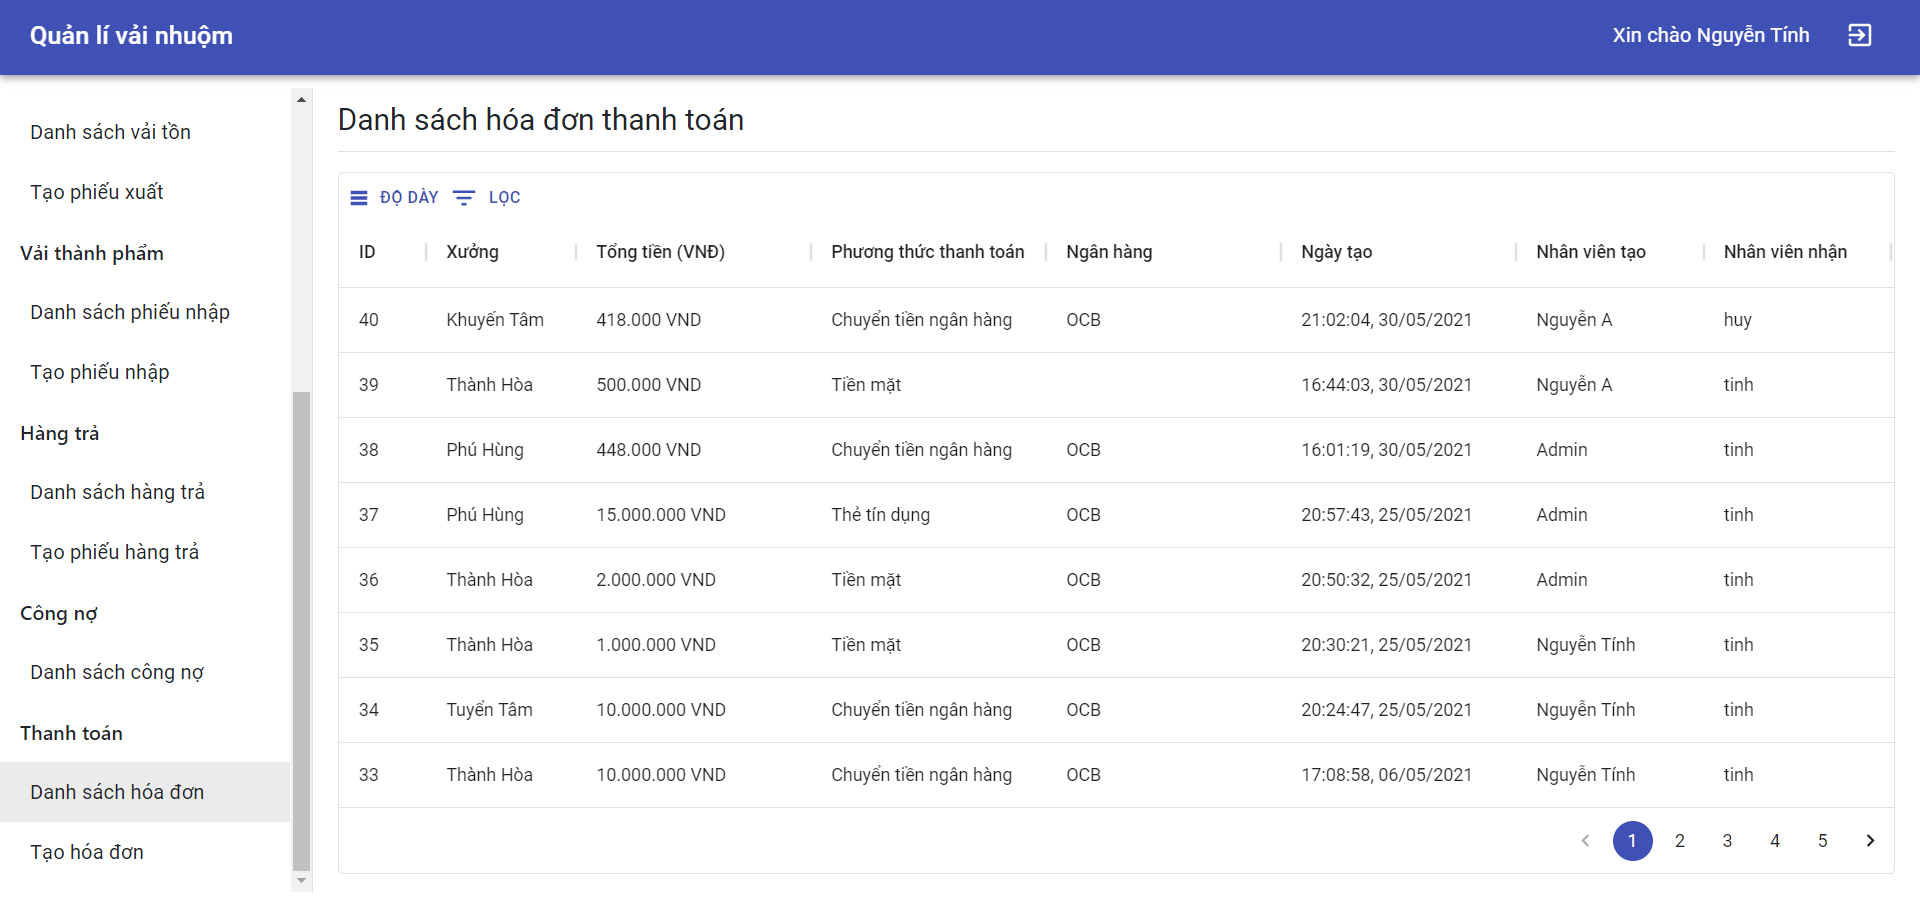
\includegraphics[width=14cm]{Image/result/danh_sach_hoa_don_thanh_toan.png}}
        \caption{Giao diện trang Danh sách hóa đơn thanh toán}
        \label{result_danh_sach_hoa_don_thanh_toan}
    \end{center}
\end{figure}

\begin{figure}[H]
    \begin{center}
        \frame{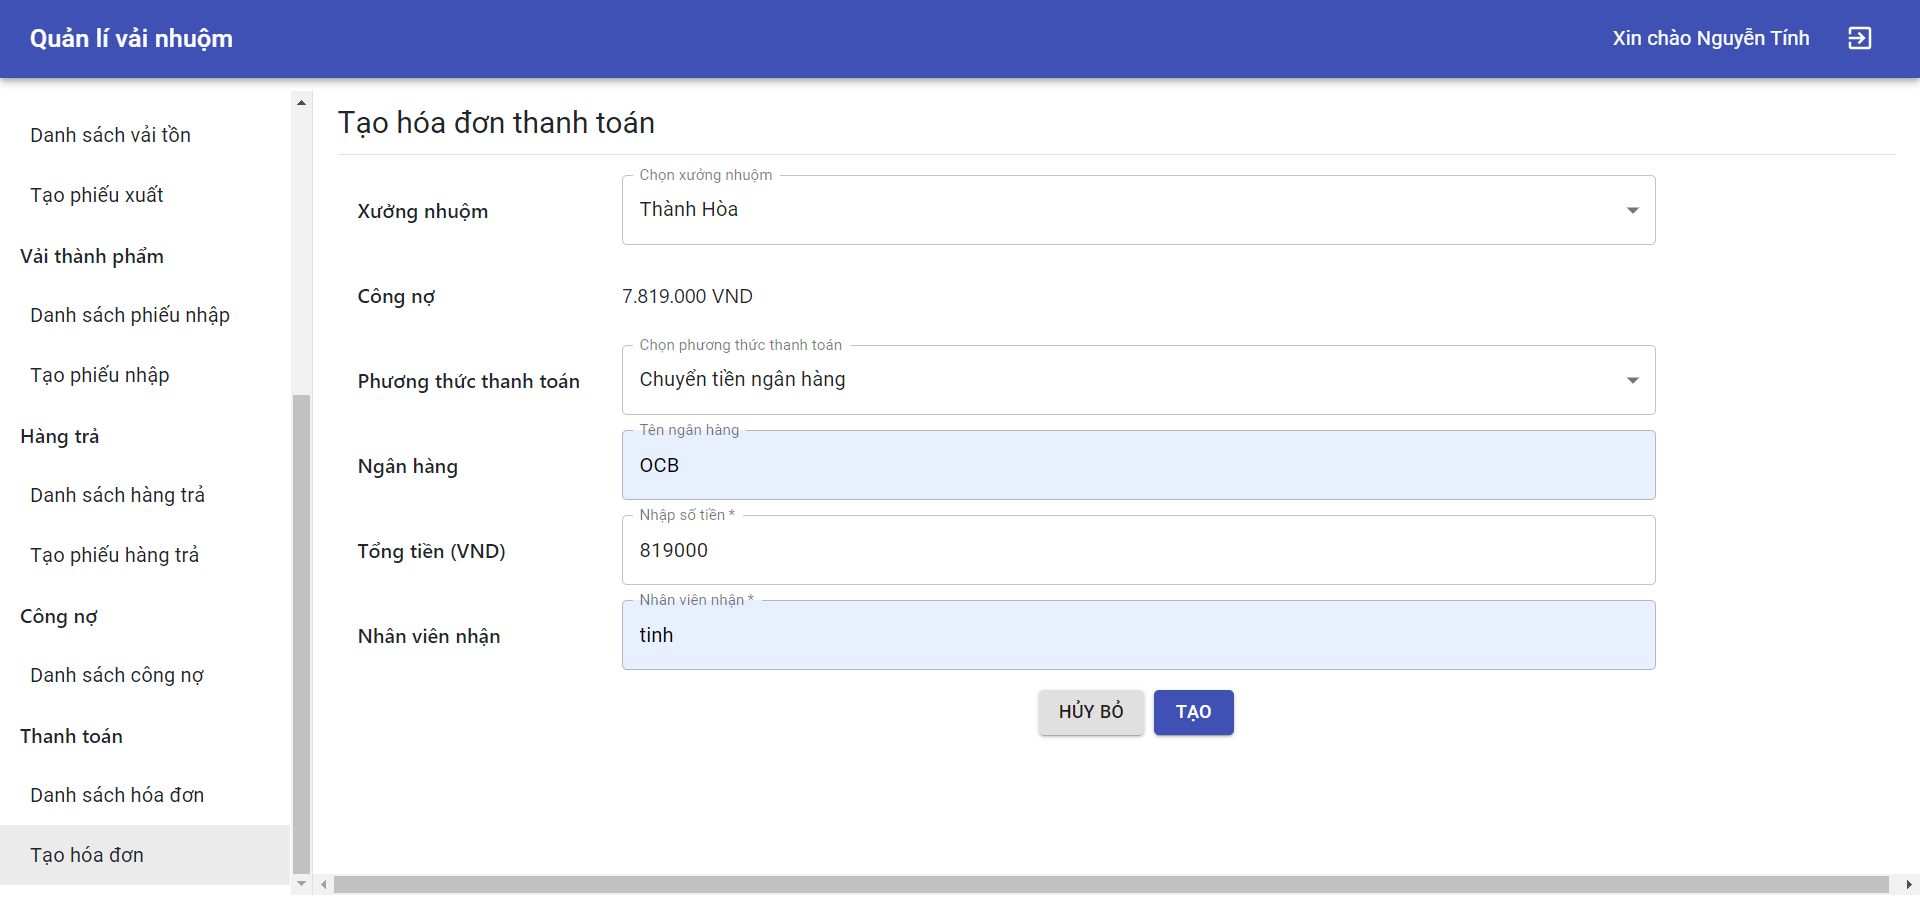
\includegraphics[width=14cm]{Image/result/tao_hoa_don_thanh_toan.png}}
        \caption{Giao diện trang Tạo hóa đơn thanh toán}
        \label{result_tao_hoa_don_thanh_toan}
    \end{center}
\end{figure}

%%%%%%%%%%%%%%%%%%%%%%%%
\textbf{Nhóm chức năng của Quản lí}

Với người dùng là Quản lí sẽ có thêm một số chức năng nâng cao, bao gồm xem danh sách các người dùng hiện tại của hệ thống [Hình \ref{result_danh_sach_nhan_vien}], tạo một người dùng mới [Hình \ref{result_tao_nhan_vien}], và tạo một xưởng nhuộm mới [Hình \ref{result_tao_xuong_nhuom}].

\begin{figure}[H]
    \begin{center}
        \frame{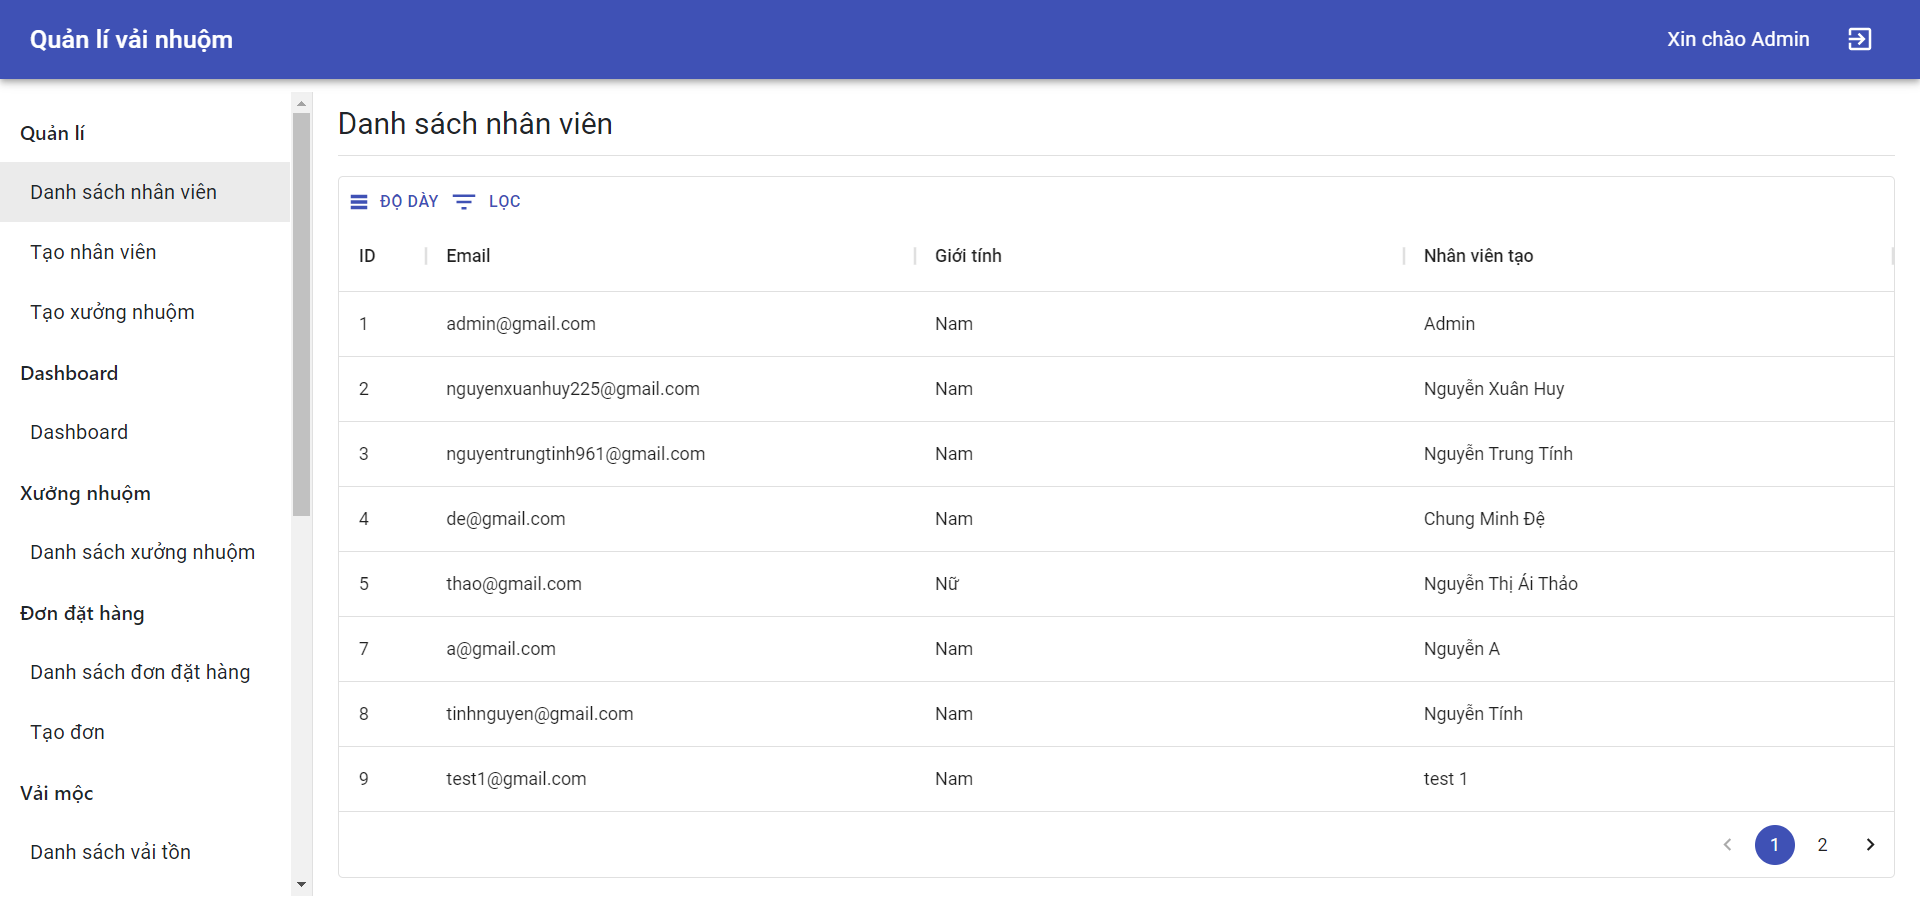
\includegraphics[width=14cm]{Image/result/danh_sach_nhan_vien.png}}
        \caption{Giao diện trang Danh sách nhân viên}
        \label{result_danh_sach_nhan_vien}
    \end{center}
\end{figure}

\begin{figure}[H]
    \begin{center}
        \frame{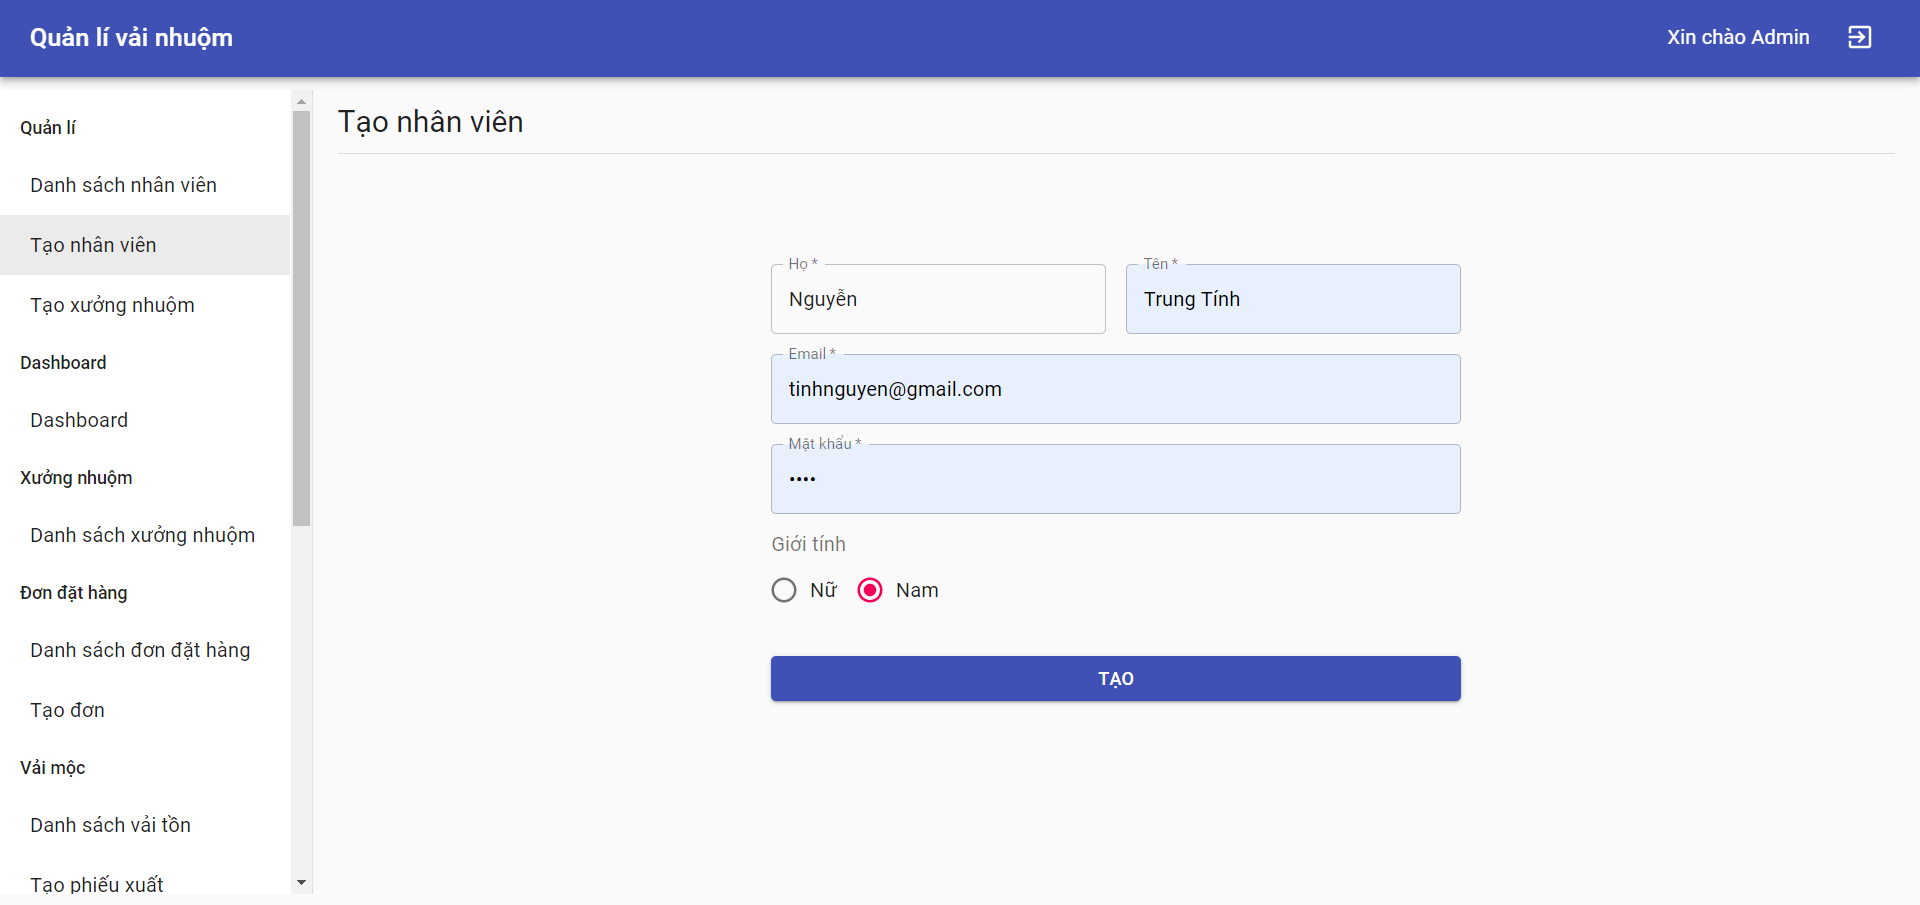
\includegraphics[width=14cm]{Image/result/tao_nhan_vien.png}}
        \caption{Giao diện trang Tạo nhân viên}
        \label{result_tao_nhan_vien}
    \end{center}
\end{figure}

\begin{figure}[H]
    \begin{center}
        \frame{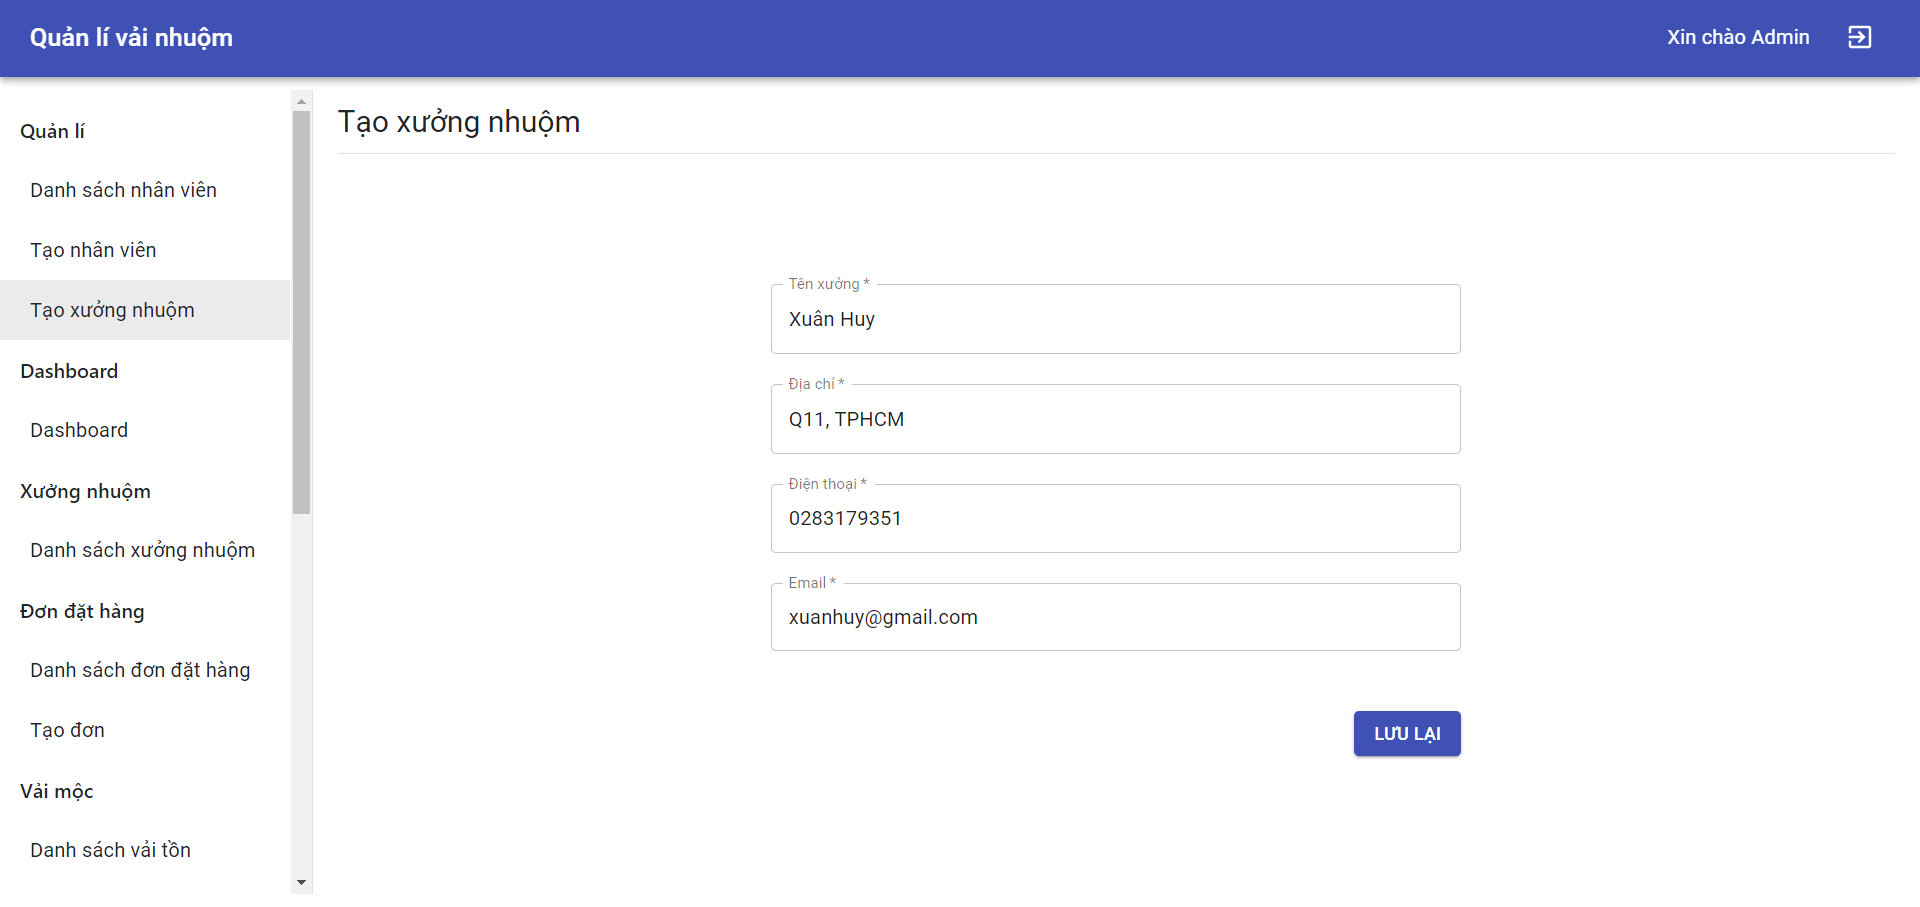
\includegraphics[width=14cm]{Image/result/tao_xuong_nhuom.png}}
        \caption{Giao diện trang Tạo xưởng nhuộm}
        \label{result_tao_xuong_nhuom}
    \end{center}
\end{figure}

% %%%%%%%%%%%%%%%%%%%%%%%%
% \textbf{}

% \begin{figure}[H]
%     \begin{center}
%         \frame{\includegraphics[width=14cm]{Image/result/}}
%         \caption{Giao diện trang}
%         \label{result_}
%     \end{center}
% \end{figure}